\documentclass[mathserif]{beamer}
\usepackage{subfigure}
\usepackage{listings}
\usepackage{courier}
\definecolor{lightlightgray}{gray}{0.95}
\definecolor{lightlightblue}{rgb}{0.4,0.4,0.95}
\definecolor{lightlightgreen}{rgb}{0.8,1,0.8}
\lstset{language=C++,
           frame=single,
           basicstyle=\ttfamily\footnotesize,
           keywordstyle=\color{black}\textbf,
           backgroundcolor=\color{lightlightgray},
           commentstyle=\color{blue},
           frame=single
           }
\usetheme[secheader]{pecostalk}
\usepackage{bibentry}
\nobibliography*
\graphicspath{{figs/}}                                                                                                                              

% defines newblock as null, giving compile issues otherwise
\let\newblock\relax 

\newcommand{\eqdef}{\stackrel{\text{\tiny def}}{=}}

\newcommand{\NVRvect}[1]{\ensuremath\boldsymbol{#1}}
\newcommand{\vect}[1]{\ensuremath\boldsymbol{#1}}
\newcommand{\NVRtensor}[1]{\NVRvect{#1}}
%\newcommand{\NVRtensor}[1]{\underline{\NVRvect{#1}}}
\newcommand{\NVRnorm}[1]{\left|\left|#1\right|\right|}
\newcommand{\norm}[1]{\left|\left|#1\right|\right|}
\newcommand{\NVRgrad}{\nabla}
\newcommand{\NVRdiv}{\NVRgrad \cdot}
\newcommand{\NVRpd}[2]{\frac{\partial#1}{\partial#2}}
\newcommand{\NVRpdd}[2]{\frac{\partial^2#1}{\partial#2^2}}
\newcommand{\NVReqdef}{\stackrel{\text{\tiny def}}{=}}

\newcommand{\NVRHgrad}{H(\text{grad})}
\newcommand{\NVRHdiv}{H(\text{div})}
\newcommand{\NVRsumm}[2]{\ensuremath\displaystyle\sum\limits_{#1}^{#2}}
 
\newcommand{\NVRcurl}{\nabla \times}
\newcommand{\NVRHcurl}{\ensuremath H(\text{curl})}

\newcommand{\code}[1]{\texttt{#1}}
\newcommand{\deal}{\code{deal.II}\,}

\newcommand{\pecosbold}[1]{{\color{pecos2}{#1}}}
\newcommand{\pecosreallybold}[1]{{\color{pecos6}{#1}}}

\newcommand{\FootSize}{\scriptsize}

\DeclareMathOperator*{\argmin}{arg\,min}

\date{August 30, 2012}
\author[Nathan V. Roberts]{Nathan V. Roberts \\
Supervisors: Leszek Demkowicz, Robert Moser \\
Committee: Todd Arbogast, George Biros, Thomas Hughes, Venkatramanan Raman
}
\institute{Institute for Computational and Engineering Sciences\\
The University of Texas at Austin}
\title[DPG for Incompressible Flow]{A Discontinuous Petrov-Galerkin Methodology\\ for Incompressible Flow}
\subtitle{Towards Automatic, Robust Mesh Adaptivity}

\begin{document}
\begin{frame}
%\begin{center}
%
\includegraphics[width=.8\linewidth]{grand_logo}\\
%\end{center}
\titlepage
%\begin{flushright}
%
\includegraphics[scale=0.1]{asc_logo}\\
%\end{flushright}
\end{frame}

%===============================================================================
% ACKNOWLEDGEMENTS
%===============================================================================
%\begin{frame}
%\frametitle{Acknowledgments}
%
%Collaborators:
%\begin{itemize}
%\item Leszek Demkowicz (UT/PECOS)
%\item Denis Ridzal (Sandia/CSRI)
%\item Pavel Bochev (Sandia/CSRI)
%\item Jesse Chan (UT/PECOS)
%\end{itemize}
%
%Support:
%\begin{itemize}
%\item Sandia (summer internships)
%\item PECOS (GRA funding)
%\item ICES (CSEM Fellowship)
%\end{itemize}
%
%\end{frame}


\begin{frame}
\frametitle{Motivation}

Incompressible flows:
\begin{itemize}
\item arise in a variety of applications, from hydraulics to aerodynamics
\item Navier-Stokes equations are of fundamental physical and mathematical interest:

\begin{itemize}
\item believed to hold the key to understanding turbulence
\item precise conditions for existence and uniqueness of solutions remain unknown (Millennium Prize problem)
\end{itemize}

\end{itemize}
%\hspace{1cm} 
\begin{center}
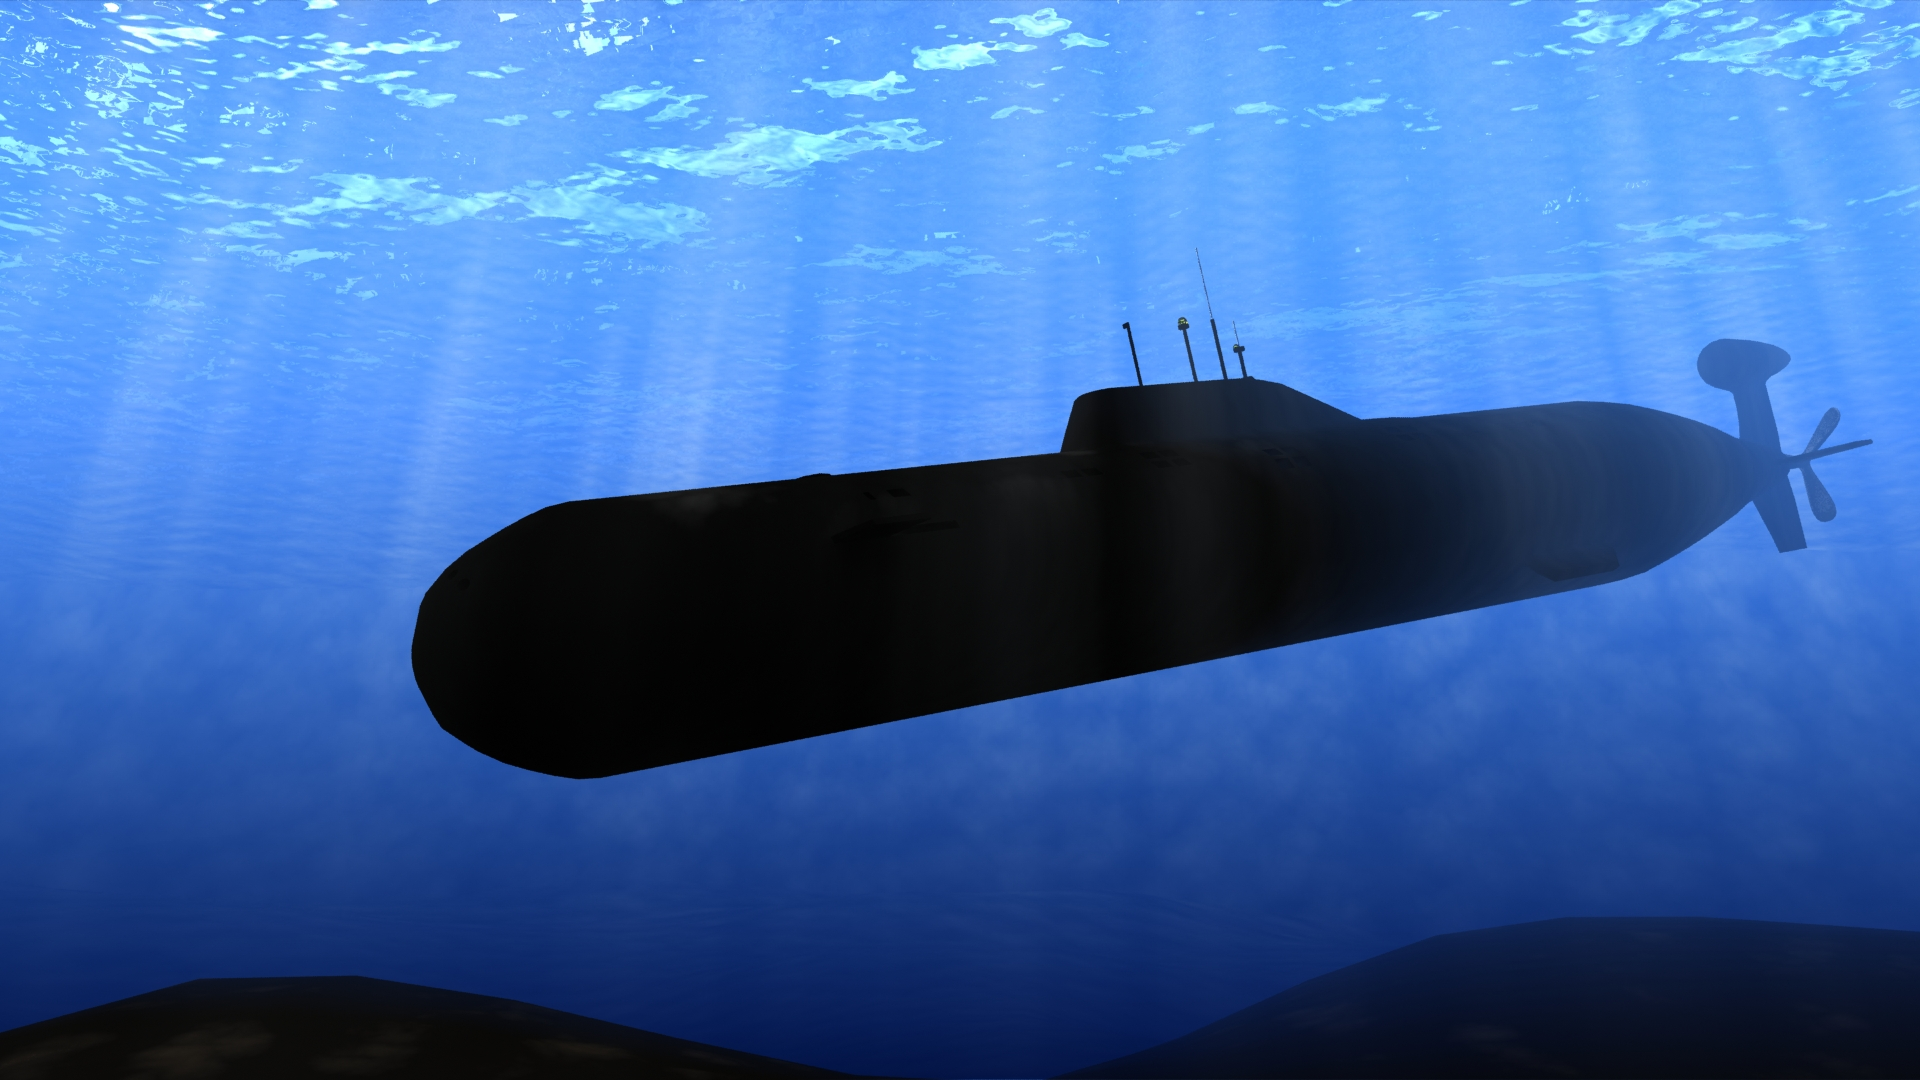
\includegraphics[width=6cm]{../figures/submarine}
\end{center}
% \hfill 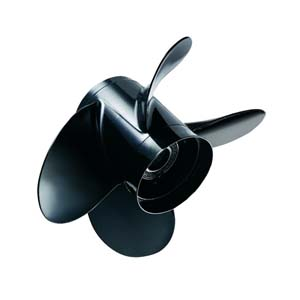
\includegraphics{../figures/propeller}\hspace{1cm}
\end{frame}

\begin{frame}
\frametitle{Motivation}

\begin{center}\nocite{Williamson1996}
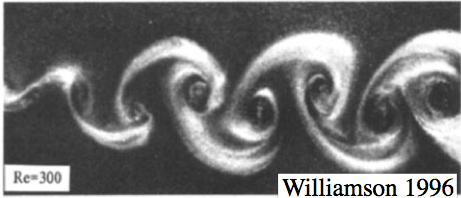
\includegraphics[scale=.5]{../figures/cylinderWakeRe300Williamson.png}\\
\end{center}

Typical solutions of incompressible flow problems involve both fine- and large-scale phenomena.

\begin{center}
$\implies$
\end{center}

A \pecosbold{uniform} finite element mesh of sufficient granularity is
\begin{itemize}
\item \pecosbold{wasteful} of computational resources, or
\item \pecosbold{infeasible} because of resource limitations.
\end{itemize}

\vspace{3mm}
\begin{center}
Therefore, an \pecosbold{adaptive mesh} is required.
\end{center}

\end{frame}

\begin{frame}
\frametitle{Motivation}
In industry:
\begin{itemize}
\item adaptivity schemes used are ad hoc, requiring a domain expert to predict features of the solution,
\item a badly chosen mesh may take considerably longer to converge or fail to converge, and
\item typically, the Navier-Stokes solve will be just one component in an optimization loop $\implies$ any failure requiring human intervention is costly.
\end{itemize}

\begin{center}
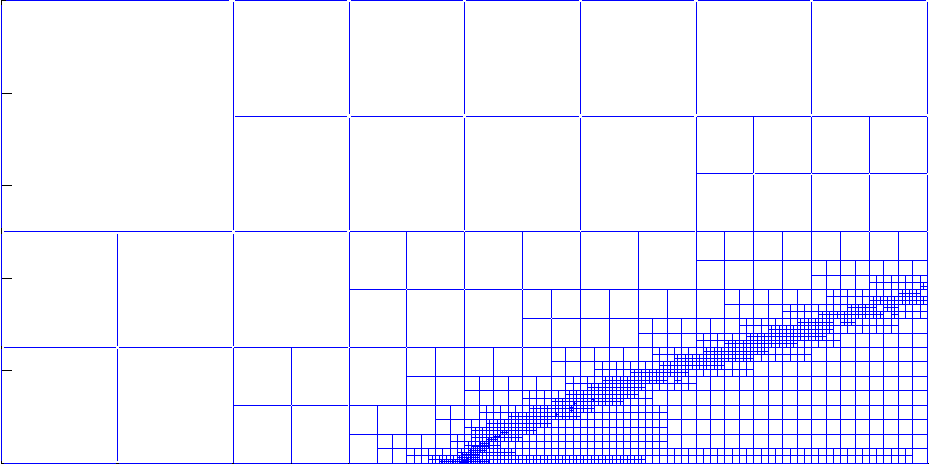
\includegraphics[scale=0.35]{../figures/Jesse/mesh10.png}
\end{center}

\end{frame}

\begin{frame}
\vspace{5mm}
\begin{center}
\pecosbold{Goal}: Develop a solver for the incompressible Navier-Stokes equations that provides \pecosbold{robust adaptivity} starting from a coarse mesh.
\end{center}
\pause
By \pecosbold{robust}, we mean:
\begin{itemize}
\item always \pecosbold{converges} to a solution in predictable time, and
\pause
\item the adaptive scheme is \pecosbold{independent} of the problem: no special expertise required for adaptivity.
\end{itemize}

% Explain here what we mean by robust: solver always converges to a solution in predictable time, and that the adaptive scheme is independent of the problem: no special expertise is required for adaptivity.

\end{frame}

%===============================================================================
% OUTLINE
%===============================================================================

% UNCOMMENT THIS TO ADD AN OUTLINE AT THE TOP OF EACH SECTION...
%\AtBeginSection[]
%{
%  \begin{frame}<beamer>
%    \frametitle{Outline}
%    \tableofcontents[currentsection]
%  \end{frame}
%}

\begin{frame}
\frametitle{Outline}
\tableofcontents
\end{frame}

\section{DPG in Brief} % 5-6 slides
% motivate as a min-residual method
% end with the two flow chart slides
%===============================================================================
% The Abstract Problem and Minimization of the Residual
%===============================================================================
\begin{frame}
\frametitle{The Abstract Problem and Minimization of the Residual}
Take $U,V$ Hilbert.\\
\vspace{5mm}
We seek $u \in U$ such that
\[
b(u,v) = l(v) \quad \forall v \in V,
\]
where $b$ and $l$ are linear in $v$.  Define $B$ by $Bu = b(u,\cdot) \in V'$; $Bu$ is a linear functional on the test space $V$.\\
\vspace{5mm}
We seek to minimize the residual in the discrete space $U_{h} \subset U$:
\begin{align*}
u_{h} = \underset{w_{h} \in U_{h}} \argmin \,\, \frac{1}{2} \norm{Bw_{h}-l}_{V'}^{2}.
\end{align*}
\end{frame}

\begin{frame}
\frametitle{The Abstract Problem and Minimization of the Residual}
\begin{align*}
u_{h} = \underset{w_{h} \in U_{h}} \argmin \,\, \frac{1}{2} \norm{Bw_{h}-l}_{V'}^{2}.
\end{align*}

% PATTER: ``not especially easy to work with'': non-constructive; involves taking a supremum
Now, the dual space $V'$ is not especially easy to work with; we would prefer to work with $V$ itself.  Recalling that the Riesz operator $R_{V} : V \rightarrow V'$ defined by 
\begin{align*}
\langle R_{V}v, \delta v\rangle=(v,\delta v)_{V}, \quad \forall \delta v \in V,
\end{align*}
is an \emph{isometry}---$\norm{R_{V}v}_{V'} = \norm{v}_{V}$---we can rewrite the term we want
to minimize as a norm in $V$:

\begin{align*}
\frac{1}{2} \norm{Bw_{h}-l}_{V'}^{2} &= \frac{1}{2} \norm{R_{V}^{-1}\left(Bw_{h}-l\right)}_{V}^{2}\\
                                                              &= \frac{1}{2} \left(R_{V}^{-1}\left(Bw_{h}-l\right), R_{V}^{-1}\left(Bw_{h}-l\right) \right)_{V}.
\end{align*}
\end{frame}

\begin{frame}
\frametitle{The Abstract Problem and Minimization of the Residual}
We seek to minimize
\begin{align*}
\frac{1}{2} \left(R_{V}^{-1}\left(Bw_{h}-l\right), R_{V}^{-1}\left(Bw_{h}-l\right) \right)_{V}.
\end{align*}
The first-order optimality condition requires that the G\^ateaux derivative be equal to zero for minimizer $u_{h}$; assuming $B$ is linear, we have
\begin{align*}
\left(R_{V}^{-1}\left(Bu_{h}-l\right), R_{V}^{-1}B \delta u_{h} \right)_{V} = 0, \quad \forall \delta u_{h} \in U_{h}.
\end{align*}
By the definition of $R_{V}$, this is equivalent to
\begin{align*} % PATTER: use the phrase ``duality pairing''
\langle Bu_{h} - l, R_{V}^{-1}B \delta u_{h} \rangle = 0 \quad \forall \delta u_{h} \in U_{h}.
\end{align*}

\end{frame}

\begin{frame}
\frametitle{The Abstract Problem and Minimization of the Residual}
We have:
\begin{align*}
\langle Bu_{h} - l, R_{V}^{-1}B \delta u_{h} \rangle = 0 \quad \forall \delta u_{h} \in U_{h}.
\end{align*}
Now, if we identify $v_{\delta u_{h}} = R_{V}^{-1}B \delta u_{h}$ as a test function, we can rewrite this as
\begin{align*}
b(u_{h},v_{\delta u_{h}}) &= l(v_{\delta u_{h}}).
\end{align*}

Thus, the discrete solution that minimizes the residual is exactly attained by testing the original equation with appropriate test functions.  We call these \pecosbold{optimal test functions}.\footnote{\FootSize \bibentry{DPG2}}

\end{frame}

\begin{frame}
\frametitle{Evaluating Error}
The derivation prompts the definition of an \pecosbold{energy norm} on the trial space:
\[
\NVRnorm{u}_{E} \NVReqdef \NVRnorm{Bu}_{V'} = \sup_{v \in V} \frac{b(u,v)}{\NVRnorm{v}_{V}}.
\]
We can use this to define a measure of the error:
\begin{align*}
\NVRnorm{u - u_{h}}_{E} &= \NVRnorm{Bu - Bu_{h}}_{V'} \\
&=  \NVRnorm{l - Bu_{h}}_{V'} \\
&= \NVRnorm{R_{V}^{-1}\left(l - Bu_{h}\right)}_{V}.
\end{align*}
Note that all the terms in the final expression are known, so that we can \pecosbold{evaluate}, not merely estimate, the error.  This drives adaptivity.
\end{frame}

%===============================================================================
% From Strong-Form PDE to DPG Form
%===============================================================================
\begin{frame}                                                                                                                                                                          
\frametitle{From Strong-Form PDE to DPG Form}
\begin{center}
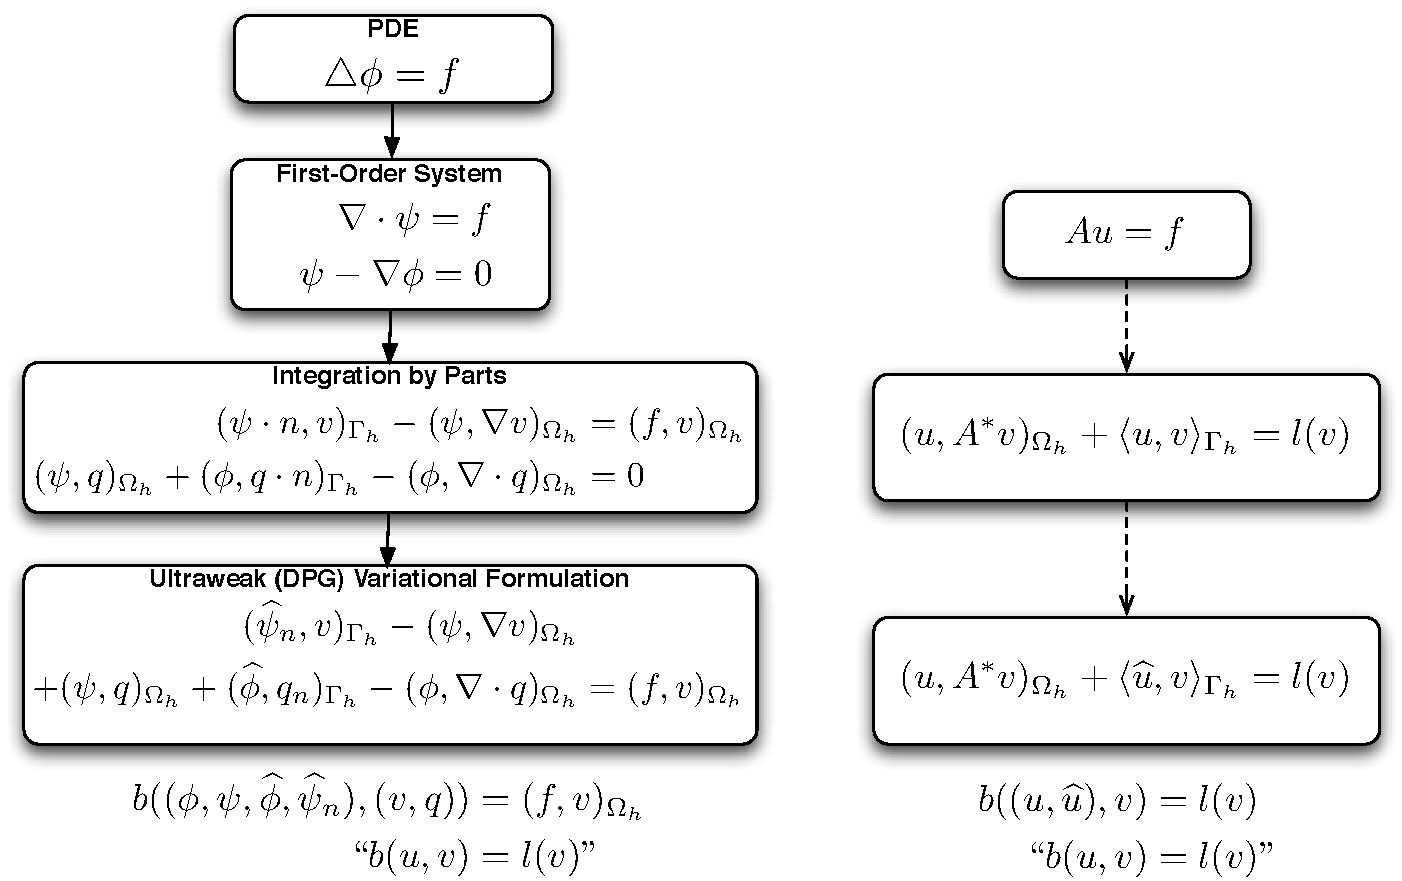
\includegraphics[width=\linewidth]{../figures/DPGFormCartoon}\\
\end{center}
\end{frame}              
%===============================================================================
% Solving with DPG
%===============================================================================
\begin{frame}                                                                                                                                                                          
\frametitle{Solving with DPG}
\begin{center} 
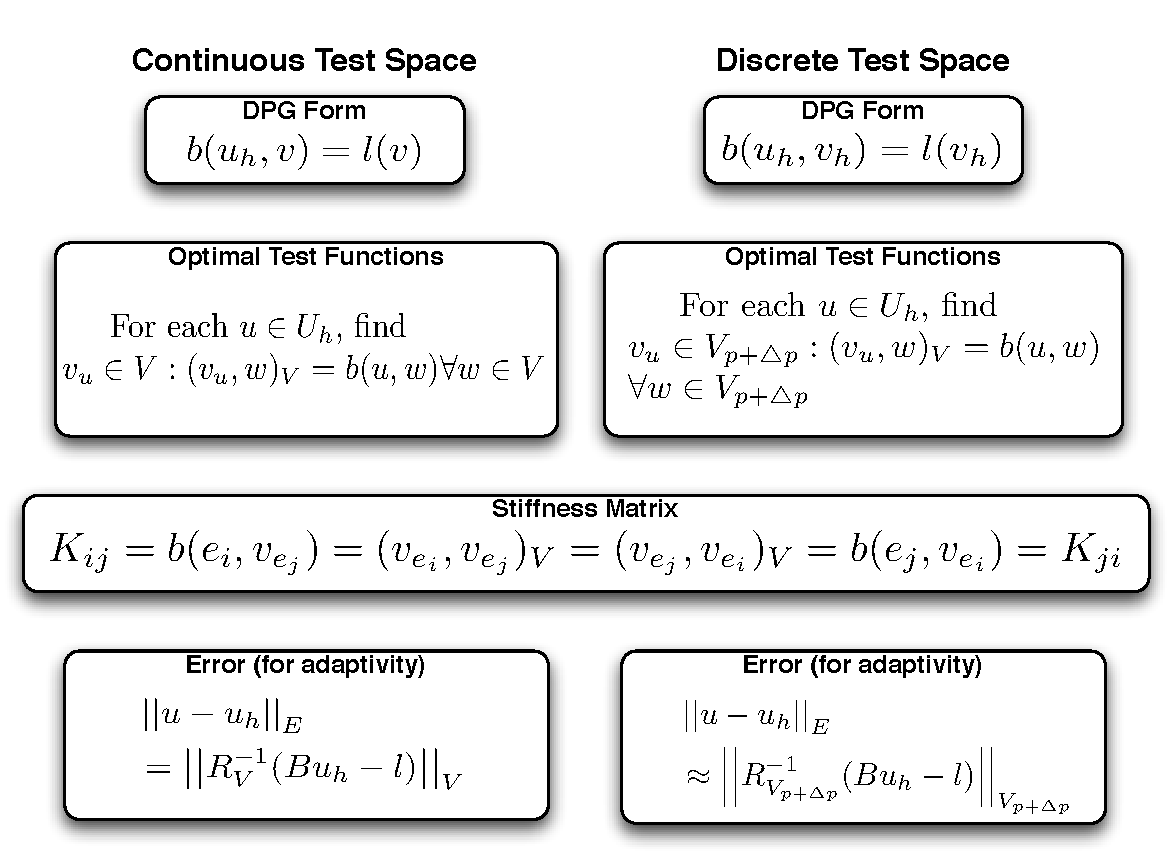
\includegraphics[width=0.9\linewidth]{../figures/DPGSolveCartoonNew}\\
\end{center}
\end{frame}


\begin{frame}
\frametitle{Graph Test Norm}

For a strong operator $A$ with formal adjoint $A^{*}$, the \pecosbold{adjoint graph space} is
\[
H_{A^{*}} = \left\{ v \in L^{2}(\Omega) : A^{*}v \in L^{2}(\Omega) \right\}
\]

and the \pecosbold{(adjoint) graph norm} on the test space $V$ is given by
\[
\NVRnorm{v}_{\rm graph} = \NVRnorm{v}_{H_{A^{*}}} = \left( \NVRnorm{v}^{2} + \NVRnorm{A^{*}v}^{2}\right)^{1/2}.
\]

\vspace{5mm}
\begin{center}
E.g. if $A^{*} = \NVRgrad$, then $H_{A^{*}} = H^{1}$, and $\NVRnorm{v}_{H_{A^{*}}} = \NVRnorm{v}_{H^{1}}$.
\end{center}
\end{frame}

\begin{frame}
\frametitle{Key Result: Well-posedness $\implies$ Optimal Convergence}
Under modest technical assumptions (true for Stokes), we have\footnote{\FootSize \bibentry{DPGStokes}}\\
\[
\NVRnorm{Au} \geq \gamma \NVRnorm{u} \implies \sup_{v \in H_{A^{*}}} \frac{b((u,\widehat{u}),v)}{\NVRnorm{v}_{H_{A^{*}}}} \geq \gamma_{\rm DPG} \left(\NVRnorm{u}^{2} + \NVRnorm{\widehat{u}}^{2}_{\widehat{H}_{A}(\Gamma_{h})}\right)^{1/2}
\]
where $\gamma_{\rm DPG} = O(\gamma)$ is a mesh-independent constant, and $\NVRnorm{\cdot}_{\widehat{H}_{A}(\Gamma_{h})}$ is the minimum energy extension norm.\\
\pause
\vspace{5mm}
By Babu\v{s}ka's Theorem,
\[
\implies \left(\NVRnorm{u - u_{h}}^{2} + \NVRnorm{\widehat{u} - \widehat{u}_{h}}^{2}_{\widehat{H}_{A}(\Gamma_{h})}\right)^{1/2} \leq \frac{M}{\gamma_{\rm DPG}} \left( {\rm B.A.E.} \right).
\]
\pause
Suffices to show that $\NVRnorm{Au} \geq \gamma \NVRnorm{u}$ to prove \pecosbold{optimal} convergence rate!
\end{frame}

\section{Equations for Incompressible Flow}
\begin{frame}
\frametitle{Incompressible Flow Equations}
\begin{center}
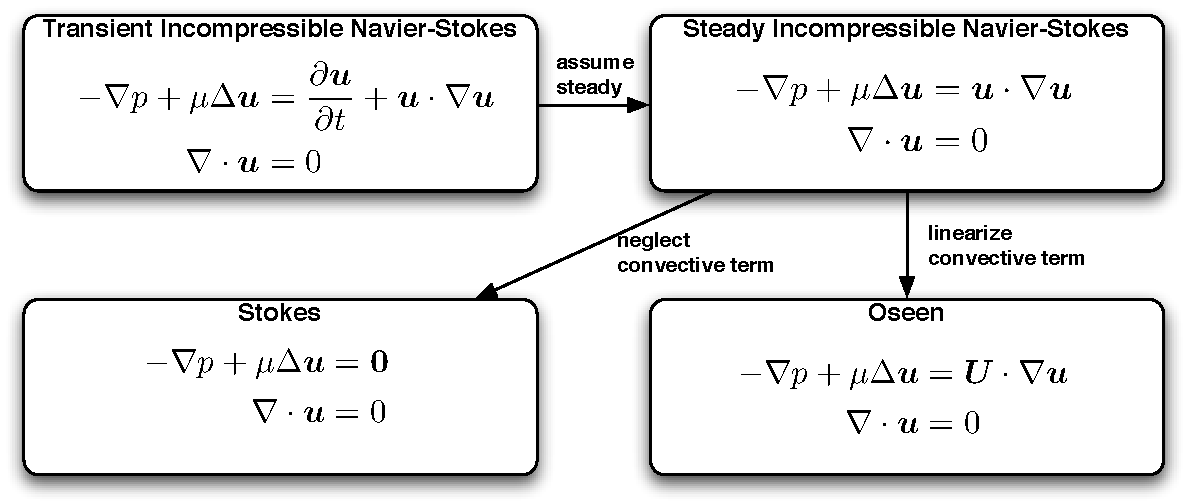
\includegraphics[width=0.9\linewidth]{../figures/incFlowEqns}\\
\end{center}
\end{frame}

\section{Stokes} % 10-12 slides
% lit. review (including various classical elements, discussion of locking and non-convergence)
% Stokes analysis, summary results
% Numerical experiments: manufactured solution, lid-driven cavity flow problem
% Probably worth mentioning the naive norm results: drives home why the analysis is valuable, and the fact that the optimal test function lives in a very specific space.
%===============================================================================
% Stokes: Classical Problem
%===============================================================================
\begin{frame}
\frametitle{Classical Stokes Problem}
The classical strong form of the Stokes problem in $\Omega \subset
\mathbb{R}^{2}$ is given by
\begin{align*}
- \mu \Delta \vect{u} + \NVRgrad p &= \vect{f} & \text{ in } \Omega, \\
\NVRdiv \vect{u} &= 0 & \text{ in } \Omega, \\
\vect{u} &= \vect{u}_D & \text{ on } \partial\Omega,
\end{align*}
where $\mu$ is viscosity, $p$ pressure, $\vect{u}$ velocity, and
$\vect{f}$ a vector forcing function.  Since by appropriate
non-dimensionalization we can eliminate the constant $\mu$, we take
$\mu=1$ throughout. 
\end{frame}
%===============================================================================
% Stokes: ``Literature Review:'' What's generally done, etc.
%===============================================================================
\begin{frame}
\frametitle{Stokes: Existing Approaches}

Naive discretizations of Stokes can exhibit \pecosbold{non-convergence} or \pecosbold{locking}.\footnote{\FootSize \bibentry{BoffiBrezziFortin}}
\\
\vspace{5mm}
Standard Galerkin discretizations:
\begin{itemize}
\item need to satisfy the \pecosbold{LBB condition}
\item examples: the MINI element, Crouzeix-Raviart element, the class of $Q_{k}-P_{k-1}$ elements
\item polynomial degree in the pressure discretization one lower than that for velocity $\implies$ pressure converges more slowly
\end{itemize}
%\item When solving saddle-point systems using Bubnov-Galerkin methods, there are two \pecosbold{Brezzi conditions} which must be satisfied.  The challenging one for Stokes is the \pecosbold{LBB condition}---much of the art of solving Stokes is to find discrete spaces that satisfy the LBB condition.%\footnote{\bibentry{BoffiBrezziFortin}}

%\item Some choices that satisfy the LBB condition are the MINI element, Crouzeix-Raviart element, and the class of $Q_{k}-P_{k-1}$ elements.  All of these require a polynomial degree in the pressure discretization one lower than that for velocity (so that pressure converges more slowly).

\end{frame}

\begin{frame}
\frametitle{Stokes: Existing Approaches}
Local discontinuous Galerkin (LDG) method:\footnote{\FootSize \bibentry{CockburnKanschatSchotzauSchwab03}}
\begin{itemize}
\item \pecosbold{locally conservative}
\item allows pressure and velocity spaces to be chosen independently
\item equal-order spaces may be used
\item convergence \emph{rate} for the pressure remains lower than that for the velocity
\end{itemize}
\end{frame}

\begin{frame}
\frametitle{Stokes: Existing Approaches}
Divergence-conforming B-splines:\footnote{\FootSize \bibentry{EvansThesis}}
\begin{itemize}
\item pointwise divergence-free space $\implies$ locally conservative
\item equal-order spaces
\item optimal convergence rates for pressure \pecosbold{and} velocity
\item non-conforming for multi-patch domains $\implies$ DG techniques for tangential continuity across patch interfaces
\end{itemize}
\end{frame}

\begin{frame}
\frametitle{DPG Applied to Stokes}

To apply DPG, we need a first-order system.  We introduce $\NVRtensor{\sigma}= \NVRgrad
\vect{u}$:
\begin{align*}
- \NVRdiv \NVRtensor{\sigma} + \NVRgrad p &= \vect{f} & \text{ in } \, \Omega, \\
 \NVRdiv \vect{u} &= 0 & \text{ in } \, \Omega, \\
 \NVRtensor{\sigma} - \NVRgrad \vect{u} &= 0 & \text{ in } \, \Omega.
\end{align*}
Testing with $(\vect{v},q,\vect{\tau})$, and integrating by parts, we have
\begin{align*}
\left(\NVRtensor{\sigma} - p \NVRtensor{I}, \NVRgrad \vect{v} \right)_{\Omega_{h}} - \left\langle \widehat{\vect{t}}_{n}, \vect{v} \right\rangle_{\Gamma_{h}} &= (\vect{f}, \vect{v} )_{\Omega_{h}}\\
\left(\vect{u}, \NVRgrad q \right)_{\Omega_{h}} -  \left\langle \widehat{\vect{u}} \cdot \vect{n}, q  \right\rangle_{\Gamma_{h}} &= 0\\
\left( \NVRtensor{\sigma}, \NVRtensor{\tau} \right)_{\Omega_{h}} + \left( \vect{u}, \NVRdiv \NVRtensor{\tau} \right)_{\Omega_{h}} - \left\langle \widehat{\vect{u}}, \NVRtensor{\tau} \vect{n}  \right\rangle_{\Gamma_{h}} &= \NVRtensor{0},
\end{align*}
where traction $\vect{t}_{n} \eqdef ( \NVRtensor{\sigma} - p \NVRtensor{I} ) \vect{n}$, and the hatted variables $\widehat{\vect{t}}_{n}$ and $\widehat{\vect{u}}$ are new unknowns representing the traces of the corresponding variables at the boundary.

\end{frame}

\begin{frame}
\frametitle{DPG Applied to Stokes}
DPG Formulation:
\begin{align*}
b(u,v) =& \left(\NVRtensor{\sigma} - p \NVRtensor{I}, \NVRgrad \vect{v} \right)_{\Omega_{h}} - \left\langle \widehat{\vect{t}}_{n}, \vect{v} \right\rangle_{\Gamma_{h}}\\
&+\left(\vect{u}, \NVRgrad q \right)_{\Omega_{h}} -  \left\langle \widehat{\vect{u}} \cdot \vect{n}, q  \right\rangle_{\Gamma_{h}}\\
&+ \left( \NVRtensor{\sigma}, \NVRtensor{\tau} \right)_{\Omega_{h}} + \left( \vect{u}, \NVRdiv \NVRtensor{\tau} \right)_{\Omega_{h}} - \left\langle \widehat{\vect{u}}, \NVRtensor{\tau} \vect{n}  \right\rangle_{\Gamma_{h}} = (\vect{f}, \vect{v} )_{\Omega_{h}} = l(v).
\end{align*}
The natural spaces for the trial variables are then:
\begin{itemize}
\item fields: $p \in L^{2}(\Omega), \vect{u} \in \vect{L}^{2}(\Omega), \NVRtensor{\sigma} \in \vect{L}^{2}(\Omega)$,
\item fluxes: $\widehat{\vect{t}}_{n} \in \NVRtensor{H}^{-1/2}(\Gamma_{h})$,
\item traces: $\widehat{\vect{u}} \in \vect{H}^{1/2}(\Gamma_{h})$.
\end{itemize}

The natural norms for fluxes and traces are \emph{minimum energy extension norms}.

\end{frame}

\begin{frame}
\frametitle{Polynomial Space Choices}
How to select polynomial spaces for $u$ and $\widehat{u}$?
\begin{itemize}
\item Graph norm $\implies$ error bounded by best approximation error.
\vspace{3mm} \pause
\item Want all variables to have same B.A.E. convergence rates.
\vspace{3mm} \pause
\item Fix polynomial order $k$ for $L^{2}$ variables.  ($k+1$ rate.)
\vspace{3mm} \pause
\item $\implies$ $k+1$ for $H^{1/2}(\Gamma_{h})$.
\vspace{3mm} \pause
\item $\implies$ $k$ for $H^{-1/2}(\Gamma_{h})$.
\end{itemize}
\end{frame}

\begin{frame}
\frametitle{Graph Test Norm}
The adjoint graph norm for our Stokes formulation is:\footnote{\FootSize \bibentry{DPGStokes}}
\begin{align*}
\norm{(\NVRtensor{\tau},\vect{v}, q)}_{\rm graph}^{2} =& \norm{\NVRdiv \NVRtensor{\tau} - \NVRgrad q}^{2} + \norm{\NVRdiv \vect{v}}^{2} + \norm{ \NVRtensor{\tau} + \NVRgrad{\vect{v}}}^{2}\\ 
&+ \norm{\NVRtensor{\tau}}^{2} + \norm{\vect{v}}^{2} + \norm{q}^{2}.
\end{align*}

\end{frame}

\begin{frame}
\frametitle{Manufactured Solution}
For our first numerical experiment (and following Cockburn et al.\footnote{\FootSize \bibentry{CockburnKanschatSchotzauSchwab03}}), we consider a manufactured solution
\begin{align*}
u_{1} &=  -e^{x} ( y \cos y + \sin y )\\
u_{2} &=  e^{x}  y \sin y\\
p &= 2 \mu e^{x} \sin y
\end{align*}
on domain $\Omega=(-1,1)^{2}$.  We use this to determine appropriate boundary conditions for the DPG problem.  We also perform an $L^{2}$ projection of the exact solution into the trial space to find the solution with the best approximation error.
\end{frame}

\begin{frame}
\frametitle{Graph Test Norm: $u_{1}$ convergence}
\begin{figure}[!htb]
\center
{\setlength{\fboxsep}{1pt}\colorbox{pecos2}{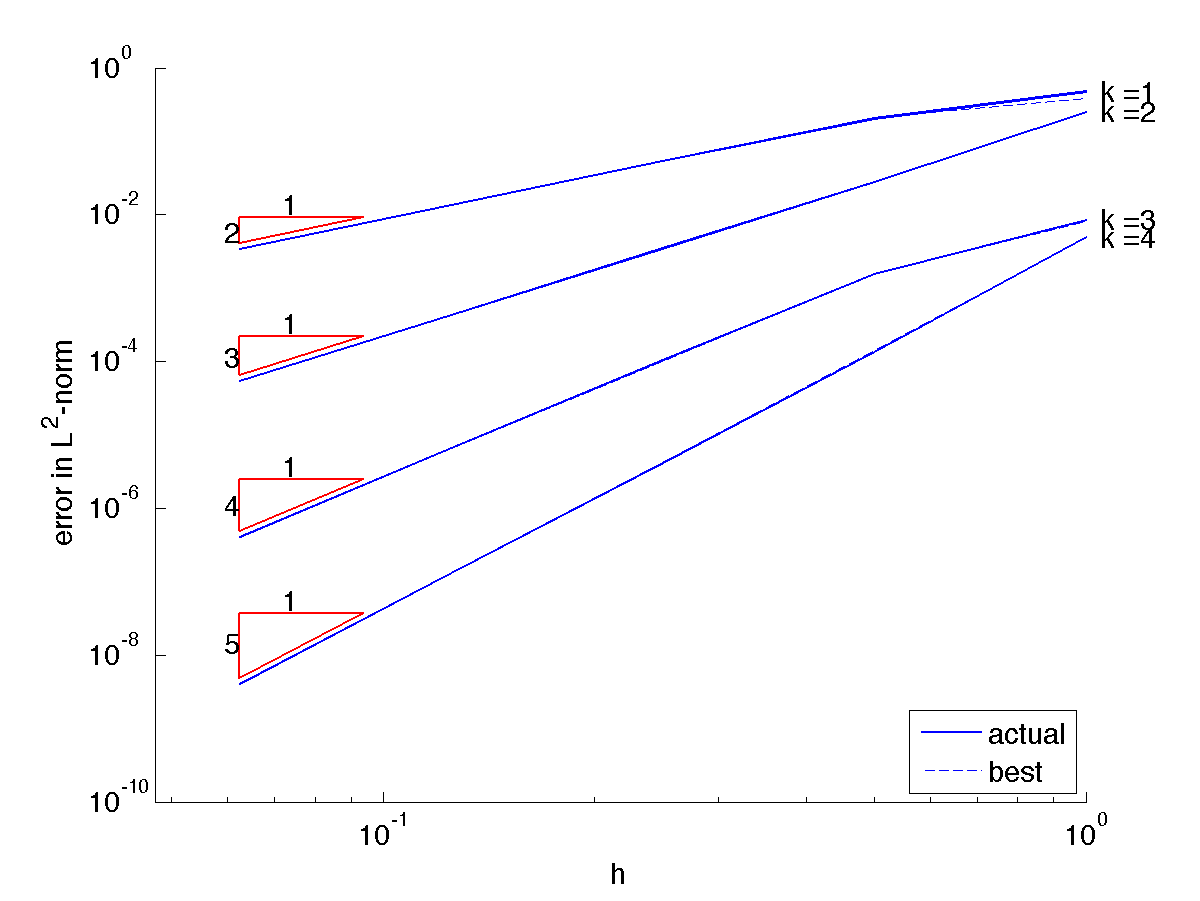
\includegraphics[scale=.38]{../figures/u1_graph_h.png}}}
\caption{$h$-convergence with the graph norm: $u_{1}$.  Dashed lines: best approximation error.}
\end{figure}
\end{frame}

\addtocounter{framenumber}{-1} % make the next frame # the same as the previous
\begin{frame}
\frametitle{Graph Test Norm: $u_{2}$ convergence}
\begin{figure}[!htb]
\center
{\setlength{\fboxsep}{1pt}\colorbox{pecos2}{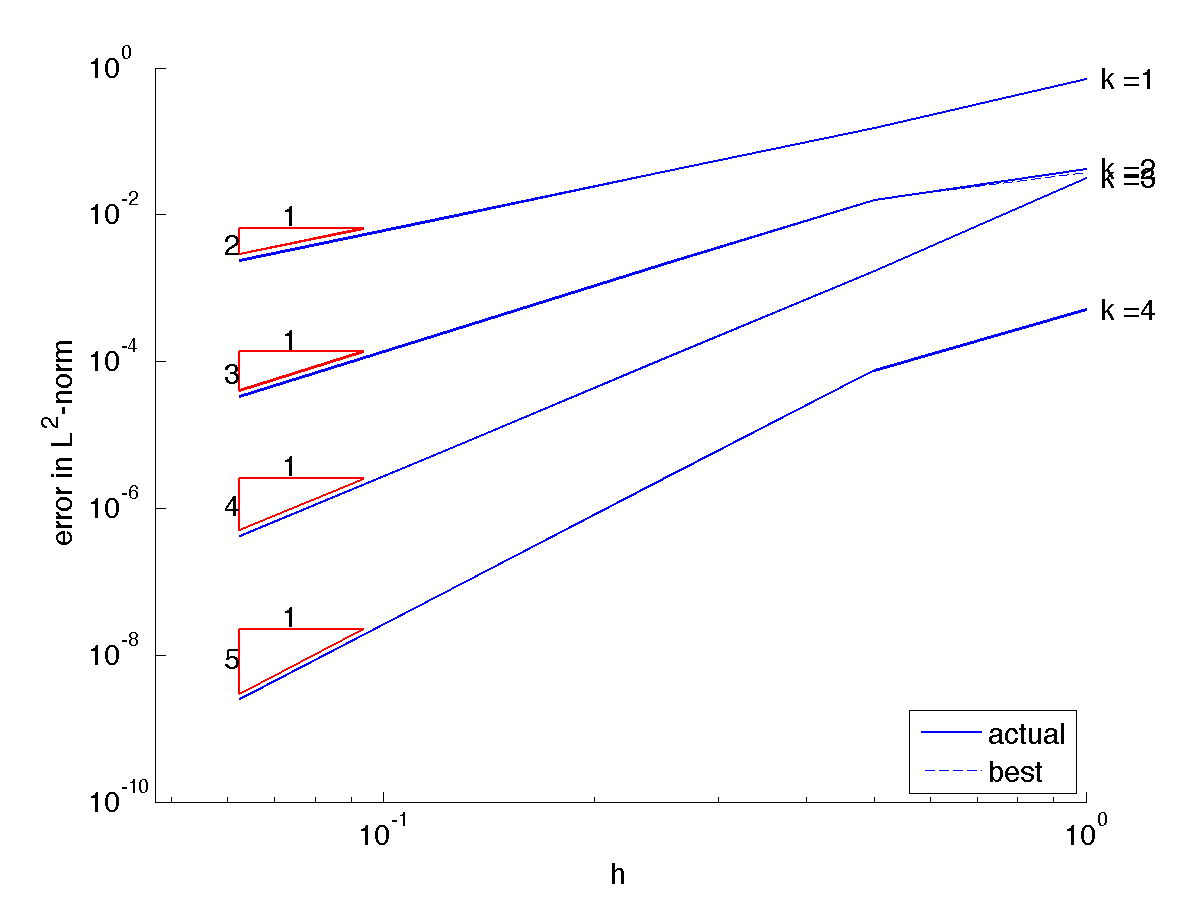
\includegraphics[scale=.38]{../figures/u2_graph_h.png}}}
\caption{$h$-convergence with the graph norm: $u_{2}$.  Dashed lines: best approximation error.}
\end{figure}
\end{frame}

\addtocounter{framenumber}{-1} % make the next frame # the same as the previous
\begin{frame}
\frametitle{Graph Test Norm: $p$ convergence}
\begin{figure}[!htb]
\center
{\setlength{\fboxsep}{1pt}\colorbox{pecos2}{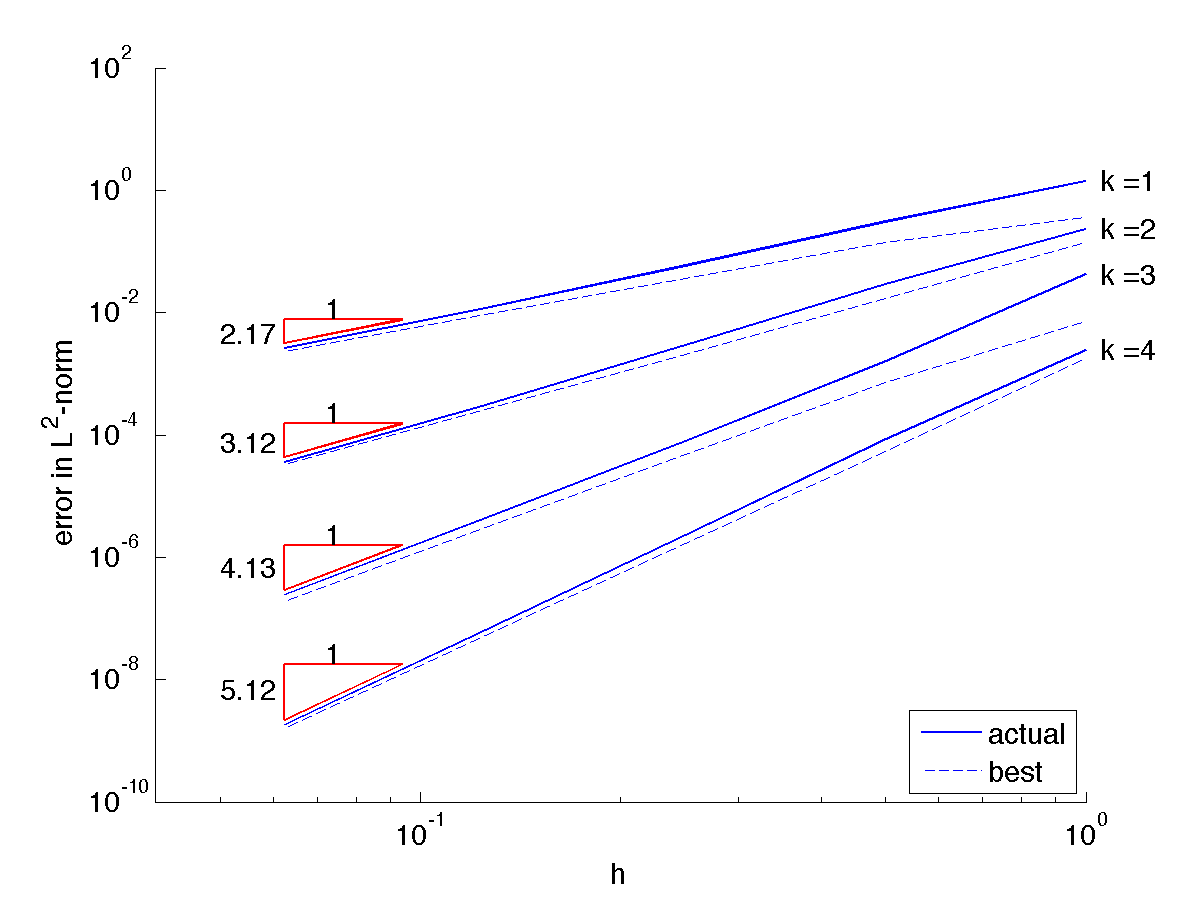
\includegraphics[scale=.38]{../figures/pressure_graph_h.png}}}
\caption{$h$-convergence with the graph norm: $p$.  Dashed lines: best approximation error.}
\end{figure}
\end{frame}

\begin{frame}
\frametitle{Naive Test Norm\footnote{\FootSize \bibentry{RobertsetAl10}}}
What if we don't use the graph norm, but a naive choice instead?

\begin{align*}
\norm{(\NVRtensor{\tau},\vect{v}, q)}_{\rm naive}^{2} = \norm{\NVRtensor{\tau}}^{2} + \norm{\NVRdiv \NVRtensor{\tau}}^{2} + \norm{\vect{v}}^{2} + \norm{\NVRgrad \vect{v}}^{2} + \norm{q}^{2} + \norm{\NVRgrad q}^{2}.
\end{align*}
\end{frame}

\begin{frame}
\frametitle{Naive Test Norm: $u_{1}$ convergence}
\begin{figure}[!htb]
\center
{\setlength{\fboxsep}{1pt}\colorbox{pecos2}{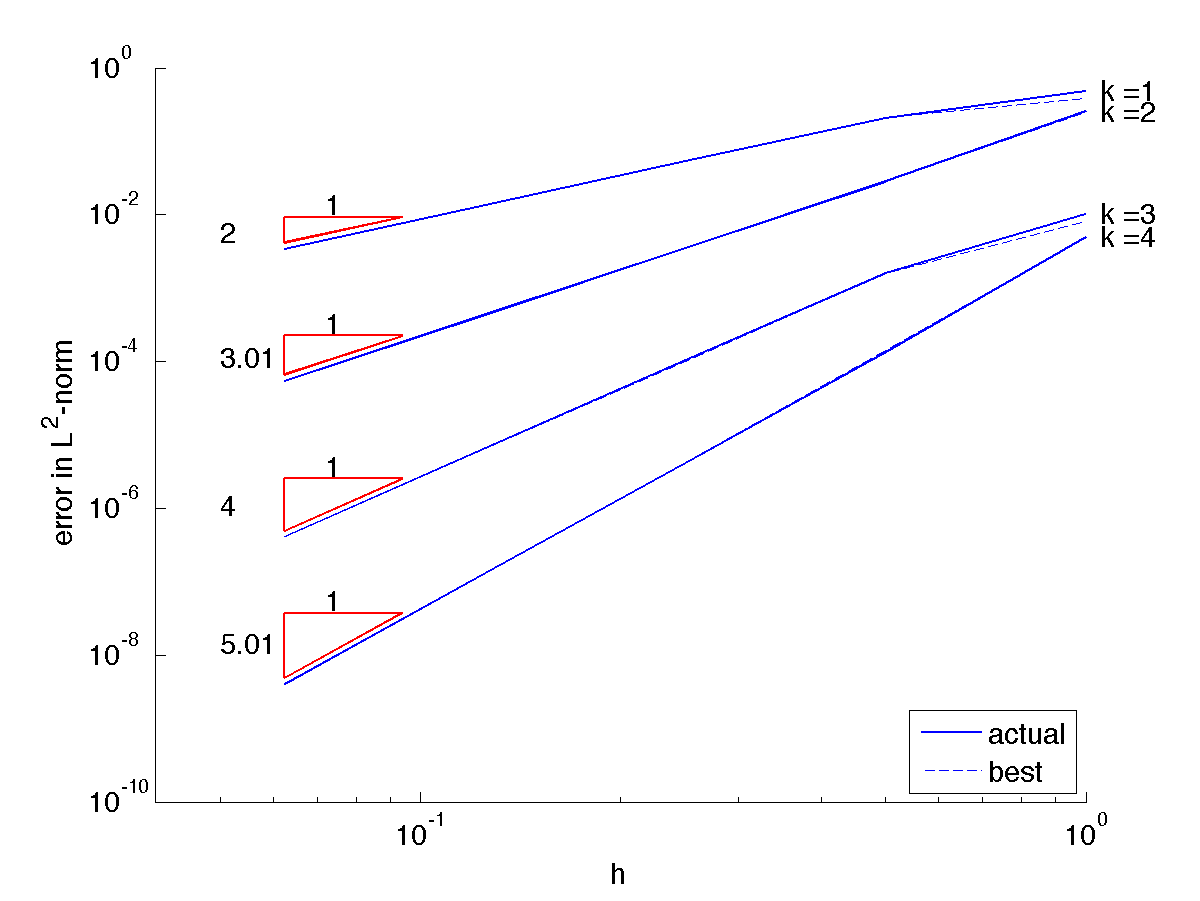
\includegraphics[scale=.38]{../figures/u1_naive_h.png}}}
\caption{$h$-convergence with the naive norm: $u_{1}$.  Dashed lines: best approximation error.}
\end{figure}
\end{frame}

\addtocounter{framenumber}{-1} % make the next frame # the same as the previous
\begin{frame}
\frametitle{Naive Test Norm: $u_{2}$ convergence}
\begin{figure}[!htb]
\center
{\setlength{\fboxsep}{1pt}\colorbox{pecos2}{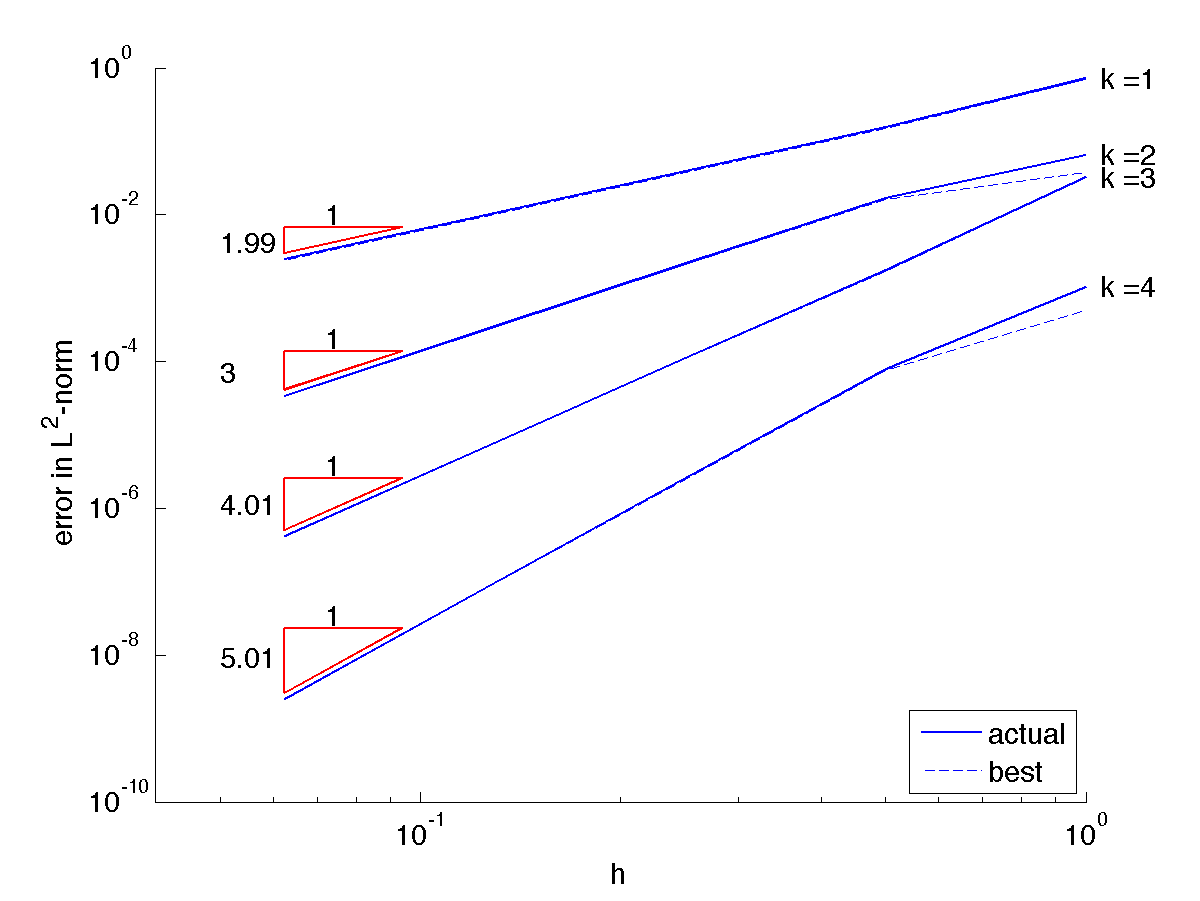
\includegraphics[scale=.38]{../figures/u2_naive_h.png}}}
\caption{$h$-convergence with the naive norm: $u_{2}$.  Dashed lines: best approximation error.}
\end{figure}
\end{frame}

\addtocounter{framenumber}{-1} % make the next frame # the same as the previous
\begin{frame}
\frametitle{Naive Test Norm: $p$ convergence}
\begin{figure}[!htb]
\center
{\setlength{\fboxsep}{1pt}\colorbox{pecos2}{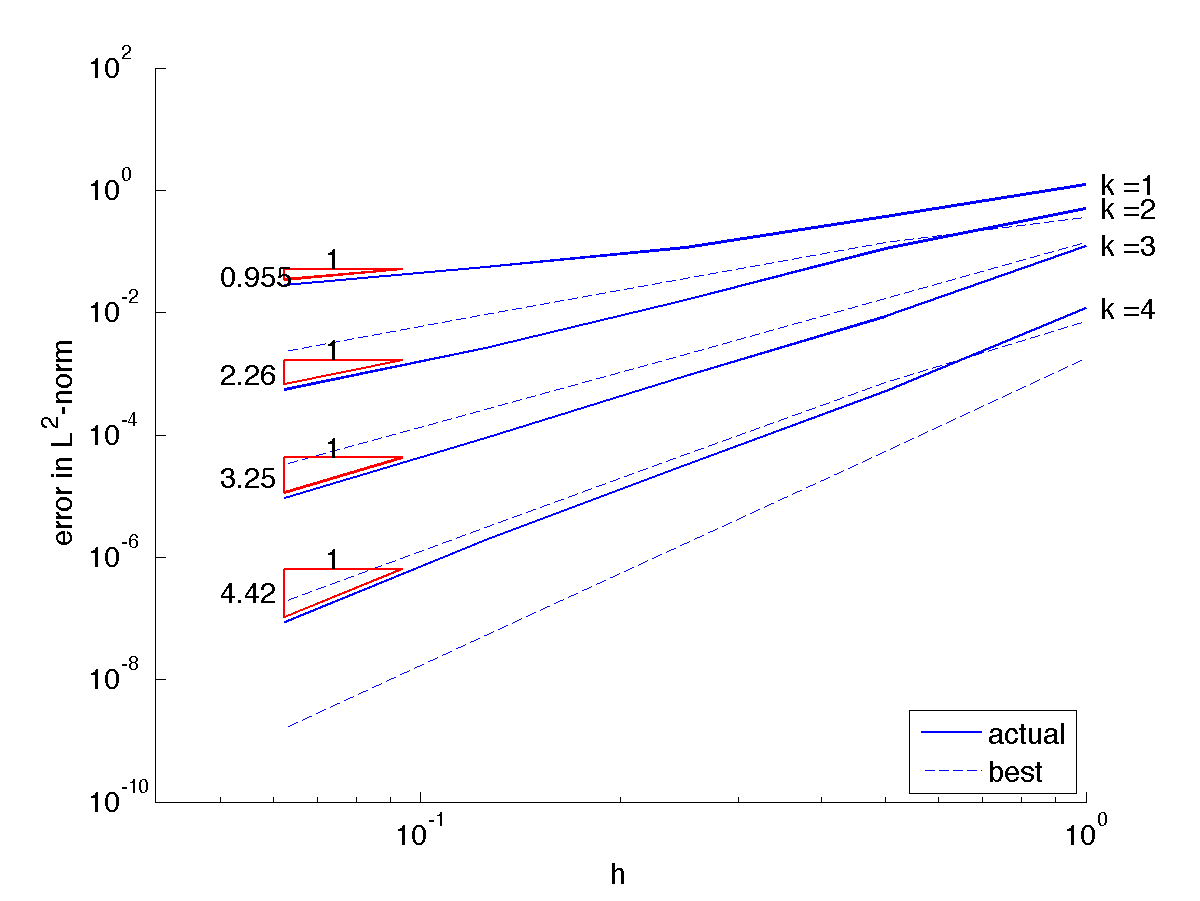
\includegraphics[scale=.38]{../figures/pressure_naive_h.png}}}
\caption{$h$-convergence with the naive norm: $p$.  Dashed lines: best approximation error.}
\end{figure}
\end{frame}

\begin{frame}
\frametitle{Graph vs. Naive Test Norm}
What's the difference between the two norms?  Why are the results better with the graph norm?

\begin{align*}
\norm{(\NVRtensor{\tau},\vect{v}, q)}_{\rm naive}^{2} =& \norm{\NVRdiv \NVRtensor{\tau}}^{2} + \norm{\NVRdiv \vect{v}}^{2} + \norm{\NVRgrad q}^{2} + \norm{\NVRtensor{\tau}}^{2} + \norm{\vect{v}}^{2} + \norm{q}^{2}\\
\vspace{30mm}
\norm{(\NVRtensor{\tau},\vect{v}, q)}_{\rm graph}^{2} =& \norm{\NVRdiv \NVRtensor{\tau} - \NVRgrad q}^{2} + \norm{\NVRdiv \vect{v}}^{2} + \norm{ \NVRtensor{\tau} + \NVRgrad{\vect{v}}}^{2}\\ 
&+ \norm{\NVRtensor{\tau}}^{2} + \norm{\vect{v}}^{2} + \norm{q}^{2}
\end{align*}
\pause
The naive norm is \pecosbold{stronger}---e.g. it requires $\NVRdiv \NVRtensor{\tau} \in L^{2}$ and $\NVRgrad q \in L^{2}$, whereas the graph norm merely requires that $\NVRdiv \NVRtensor{\tau} - \NVRgrad q \in L^{2}$.  

\end{frame}

\begin{frame}
\frametitle{Lid-Driven Cavity Flow Problem}
A classic test case for Stokes flow is the \pecosbold{lid-driven cavity flow problem}.  Consider a square cavity with an incompressible, viscous fluid, with a lid that moves at a constant rate.  The resulting flow will be vorticular; there will be \pecosbold{Moffat eddies} at the corners; in fact, the exact solution will have an infinite number of such eddies, visible at progressively finer scales.\footnote{\FootSize \bibentry{Moffat}}
\begin{center}
{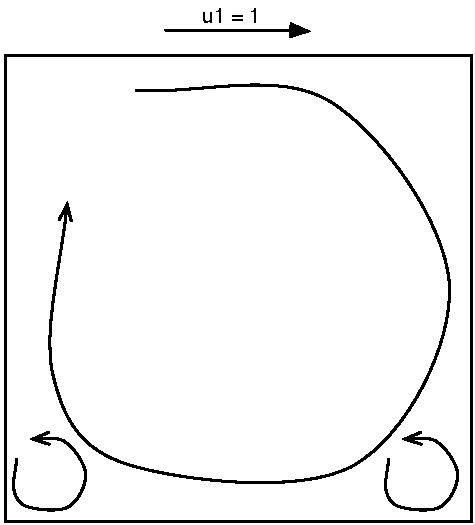
\includegraphics[scale=0.40]{../figures/cavity_flow_cartoon.pdf}}
\end{center}
\end{frame}

\begin{frame}
\frametitle{Lid-Driven Cavity Flow Problem}
\begin{center}
{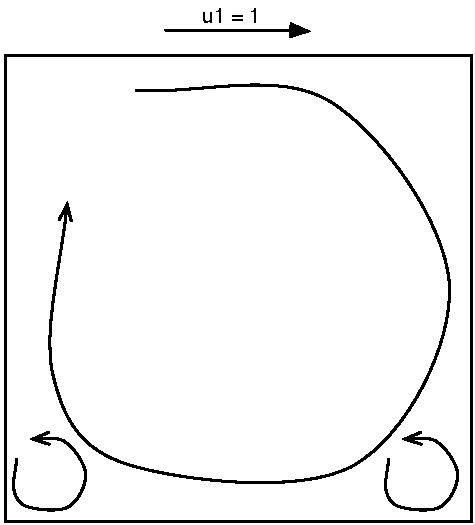
\includegraphics[scale=0.40]{../figures/cavity_flow_cartoon.pdf}}
\end{center}
\small{Because the BCs for the problem are discontinuous at the top corners, the exact solution lies outside of $H^{1}$.  So we introduce a small ``ramp'' on either side, of width $\epsilon = \frac{1}{64}$.}
\end{frame}

\begin{frame}
\frametitle{Lid-Driven Cavity Flow Problem}
Since the exact solution is unknown, we compare an overkill mesh to a series of adaptive and uniformly refined solutions.\\

\begin{itemize}
\item For all meshes, we use quadratic field variables ($k=2$).
\item Overkill mesh had $256 \times 256$ elements (5,576,706 dofs).
\item Initial adaptive mesh had $2 \times 2$ elements.
\end{itemize}
\end{frame}

\begin{frame}
\frametitle{Lid-Driven Cavity Flow: $h$-adaptivity}
\begin{figure}[!htb]
\begin{center}
{\setlength{\fboxsep}{1pt}\colorbox{pecos2}{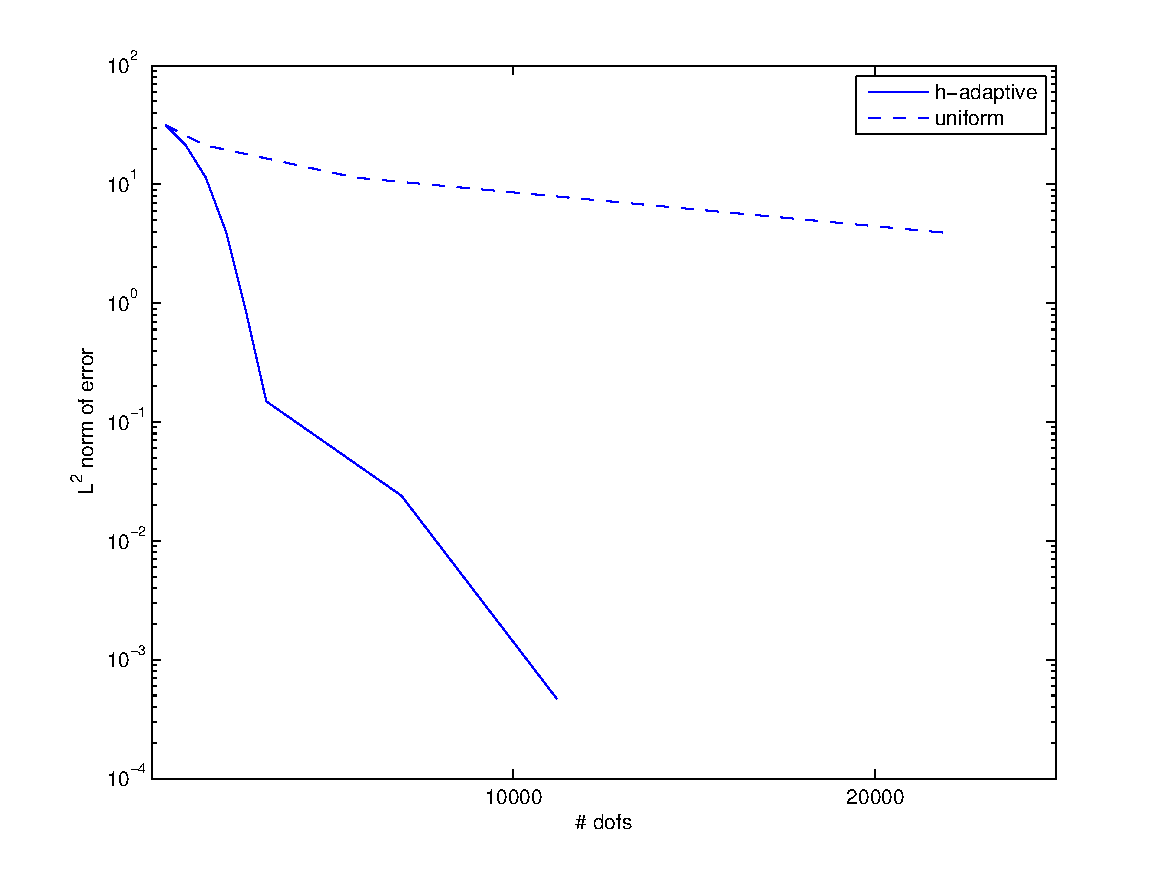
\includegraphics[scale=0.40]{../figures/adaptive_cavity_flow_quadratic_vs_overkill.pdf}}}
\end{center}
\caption{Euclidean norm of $L^{2}$ error in all field variables in $h$-adaptive mesh relative to an overkill mesh with $256 \times 256$ quadratic elements.  The Euclidean norm of the overkill solution is 6.73.}
\end{figure}

\end{frame}

\begin{frame}
\frametitle{Lid-Driven Cavity Flow: Streamlines}
\begin{center}
{\setlength{\fboxsep}{1pt}\colorbox{pecos2}{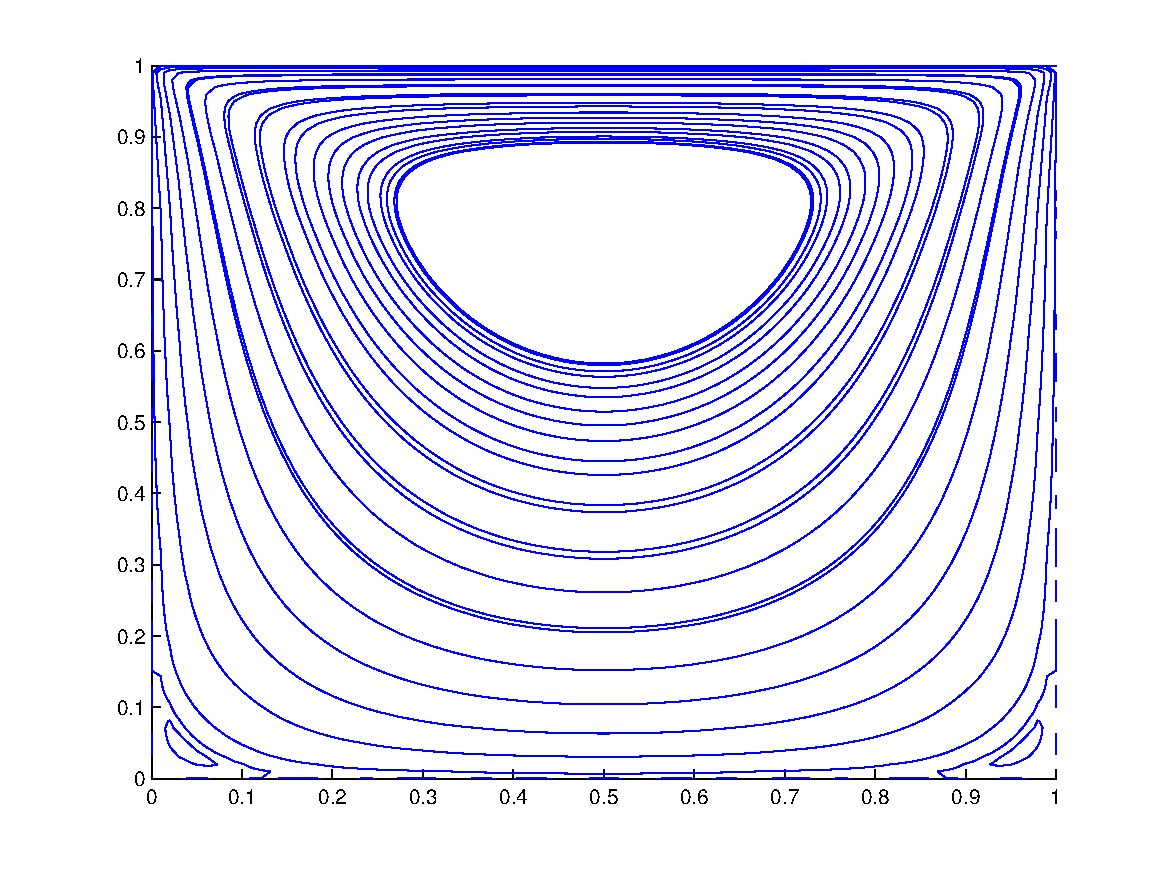
\includegraphics[scale=0.25]{../figures/streamlines_p2_r7.pdf}}} \hspace{5mm} {\setlength{\fboxsep}{1pt}\colorbox{pecos2}{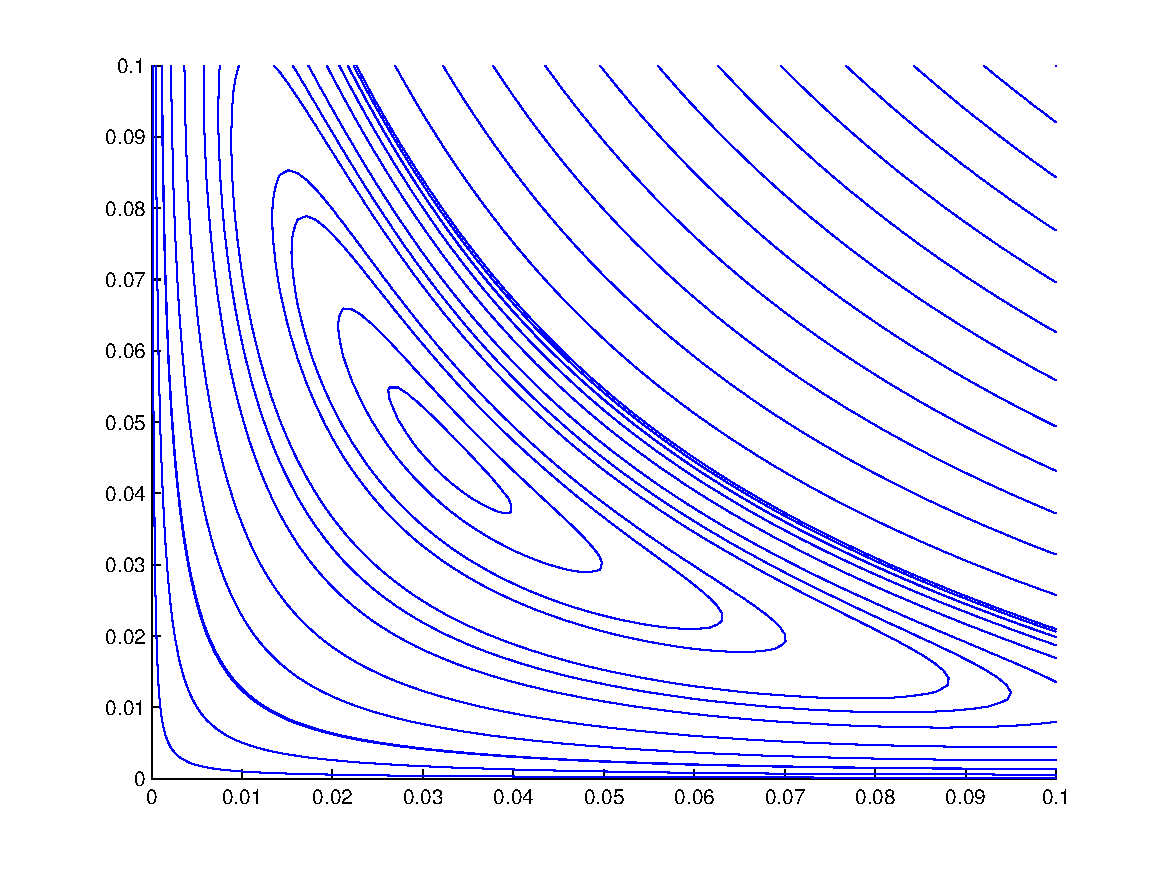
\includegraphics[scale=0.25]{../figures/streamlines_detail_p2_r7.pdf}}}
\end{center}
Streamlines for the full cavity and for the lower-left corner, on a quadratic mesh after 7 adaptive refinements.  The lower-left corner shows the first Moffat eddy.  The final mesh has 124 elements and 11,202 dofs.
\end{frame}

\begin{frame}
\frametitle{Lid-Driven Cavity Flow: Streamlines}
Using a cubic mesh and running 11 refinement steps, we can resolve the second Moffat eddy:
\begin{center}
{\setlength{\fboxsep}{1pt}\colorbox{pecos2}{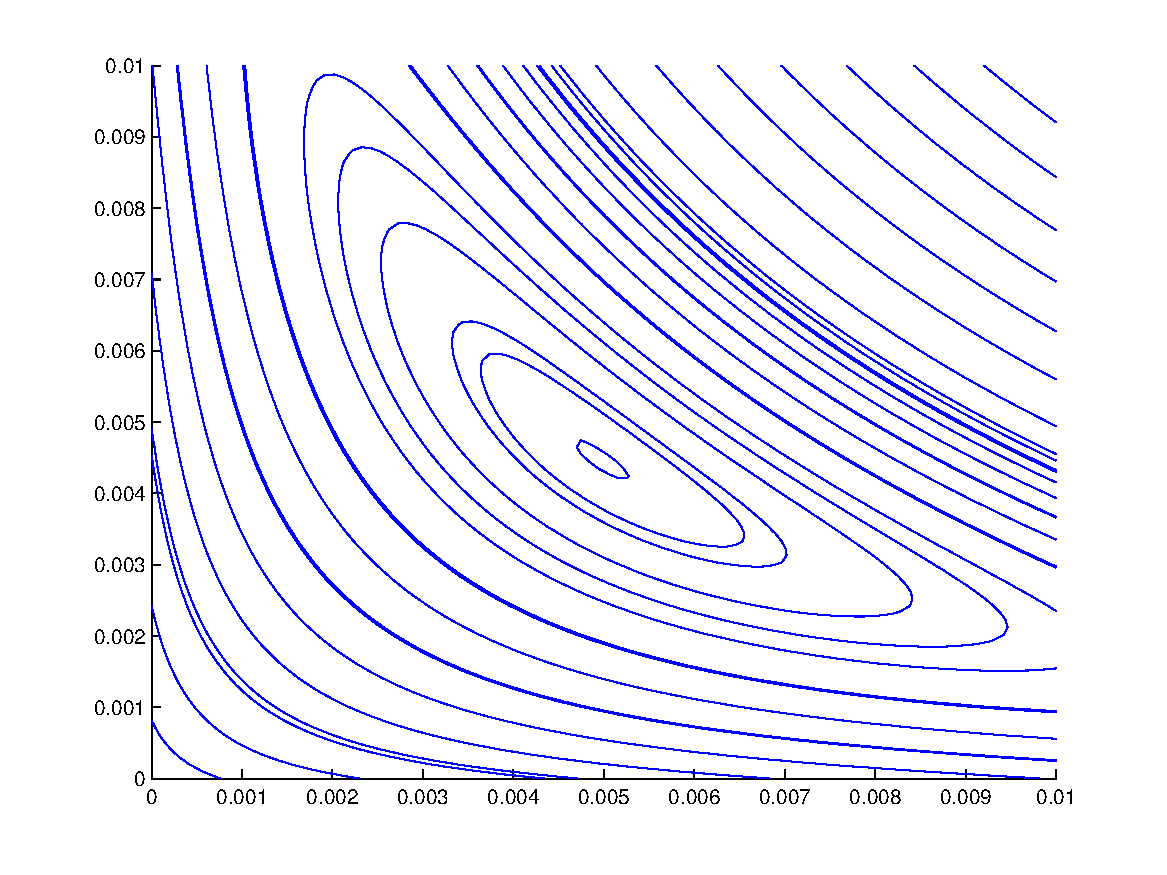
\includegraphics[scale=.35]{../figures/streamlines_minute_detail_p3_r11.pdf}}}
\end{center}
Streamlines for the lower-left corner on a cubic mesh after 11 adaptive refinements: the second Moffat eddy.  The final mesh has 298 elements and 44,206 dofs.
\end{frame}


\section{Camellia} % 10-12 slides
% lit. review: deal II, libMesh, FEniCS
% what we do, with a couple selected details
% pretty pictures of solutions produced with Camellia?
\begin{frame}
\frametitle{Camellia}
\pecosbold{Design Goal}: make DPG research and experimentation as simple as possible, without sacrificing too much by way of performance.\\

\begin{block}{Existing FEM Software}
\begin{itemize}
\item \deal\footnotemark
\item libMesh\footnotemark
\item FEniCS\footnotemark
\end{itemize}
\end{block}
\addtocounter{footnote}{-2}
\footnotetext{\FootSize \bibentry{BangerthKanschat99}}
\addtocounter{footnote}{1}
\footnotetext{\FootSize \bibentry{Kirk2006}}
\addtocounter{footnote}{1}
\footnotetext{\FootSize \bibentry{fenics:book}}
\end{frame}

\begin{frame}
\frametitle{FEM Software: \deal features}
\begin{block}{}
\begin{itemize}
\item flexible: possible to vary choices for FE spaces, spatial dimension, var. formulations, and linear solvers without too much effort
\item easy to use through encapsulation: details of complex data structures hidden from user
\item safe: runtime parameter checking allows many errors to be detected early in development
\item extensive documentation
\item \pecosbold{hypercube} topologies (lines, quads, hexahedra) supported (with several element types: CG and DG Lagrange, N\'{e}d\'{e}lec, Raviart-Thomas)
\end{itemize}
\end{block}
\end{frame}

\begin{frame}
\frametitle{FEM Software: \deal features, continued}
\begin{block}{}
\begin{itemize}
\item $h$-, $p$-, and $hp$-adaptivity
\item distributed stiffness matrix computation
\item recently added: distributed mesh storage\footnotemark
\end{itemize}
\end{block}\footnotetext{\FootSize \bibentry{dealiiwithp4est}}
\end{frame}

\begin{frame}
\frametitle{FEM Software: libMesh and FEniCS}
\begin{block}{libMesh features}
\begin{itemize}
\item inspired by \deal
\item \code{Element} class designed for subclassing
\item many topologies provided: triangles, quads, hexahedra, tetrahedra, prisms, and pyramids
\item $h$-, $p$-, and $hp$-adaptivity
\item distributed stiffness matrix computation
\end{itemize}
\end{block}

\begin{block}{FEniCS features}
\begin{itemize}
\item aim: highly automated solution of FE problems
\item emphasis is on simplicity, especially in specification of variational forms
\item simplex topologies (intervals, triangles, tetrahedra) supported
\end{itemize}
\end{block}
\end{frame}

\begin{frame}
\frametitle{Camellia\footnote{\FootSize \bibentry{RobertsetAl11}}}
\pecosbold{Design Goal}: make DPG research and experimentation as simple as possible, without sacrificing too much by way of performance.
\vspace{3mm}
\begin{center}
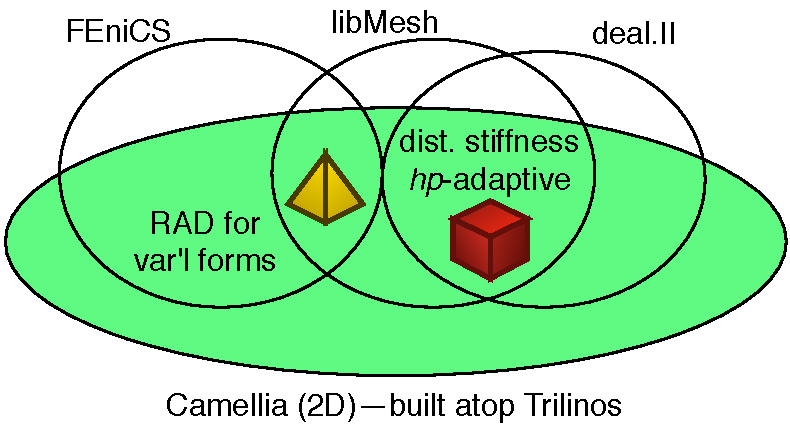
\includegraphics[scale=.65]{../figures/CamelliaVennDiagram.pdf}
\end{center}
%\begin{block}{}
%\begin{itemize}
%\item Like \deal and libMesh, support $hp$-adaptive hierarchical meshes
%\item Like libMesh, support multiple element types (quads and triangles in 2D)
%\item Like FEniCS, support rapid development of variational forms
%\item Leverage existing software by building atop Trilinos\footnotemark
%\end{itemize}
%\end{block}
\addtocounter{footnote}{1}
\footnotetext{\FootSize \bibentry{TrilinosShortAuthors}}
\end{frame}

%\begin{frame}
%\frametitle{Camellia\footnote{\FootSize \bibentry{RobertsetAl11}}}
%\pecosbold{Design Goal}: make DPG research and experimentation as simple as possible, without sacrificing too much by way of performance.
%\begin{block}{Goals for Camellia (Achieved)}
%\begin{itemize}
%\item Make variational form and inner product easy to specify
%\item Arbitrary, $hp$-adaptive 2D meshes (quads and triangles)---including meshes of arbitrary irregularity
%\item ``Reasonable'' speed and scalability (distributed stiffness matrix computation)
%\item Support for nonlinear problems
%\end{itemize}
%\end{block}
%
%\vspace{3 mm}
%
%%\begin{figure}[h]
%%\centering
%%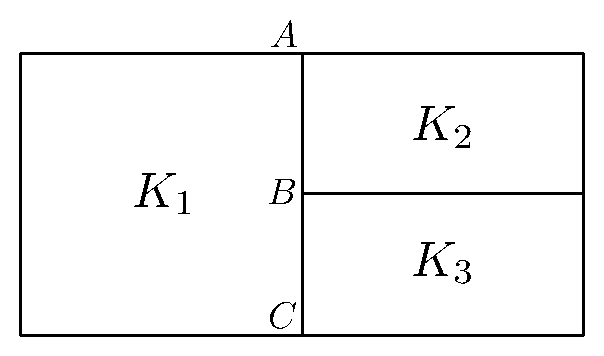
\includegraphics[scale=0.35]{../fig/hangingNode.eps}
%%\label{fig:hangingNode}
%%\end{figure}
%\end{frame}
%
%\begin{frame}
%\frametitle{Camellia}
%\begin{block}{Goals for Camellia (Aspirational)}
%\begin{itemize}
%\item Support for minimization of a \pecosbold{nonlinear} residual
%\item Support for curvilinear geometries
%\item Better scalability (distributed mesh storage)
%\item Longer term: 3D meshes
%\end{itemize}
%\end{block}
%
%\end{frame}

%===============================================================================
% WHAT INTREPID (TRILINOS) PROVIDES
%===============================================================================
\begin{frame}
\frametitle{Trilinos Support}
\begin{block}{}
\begin{center}
\begin{tabular}{l c}
\pecosbold{Feature}			&\pecosbold{Trilinos Package} \\
OO interface to MUMPS 		&Amesos \\
KLU solver 				&Amesos \\
conforming basis functions	&Intrepid \\
pullbacks/Piola transforms 	&Intrepid \\
smart multidimensional arrays 	&Intrepid \\
distributed compressed row storage matrices	&Epetra \\
cell topologies 				&Shards \\
reference-counted pointers 				&Teuchos \\
space-filling curves for spatially local mesh partitioning 		&Zoltan \\
\end{tabular}
\end{center}
\end{block}
\end{frame}

\begin{frame}
\frametitle{Camellia: Other Users}
\begin{itemize}
\item Jesse Chan: compressible Navier-Stokes
\item Truman Ellis: compressible Navier-Stokes with turbulence
\end{itemize}
\begin{figure}
\centering
\subfigure[Mesh]{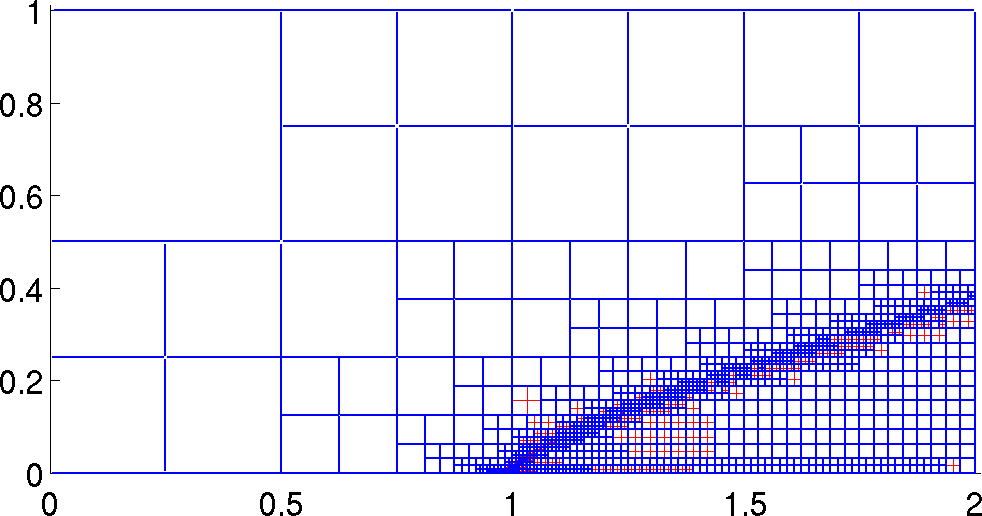
\includegraphics[height = 3cm]{../figures/Jesse/Mesh10.png}}
\subfigure[$u_1$]{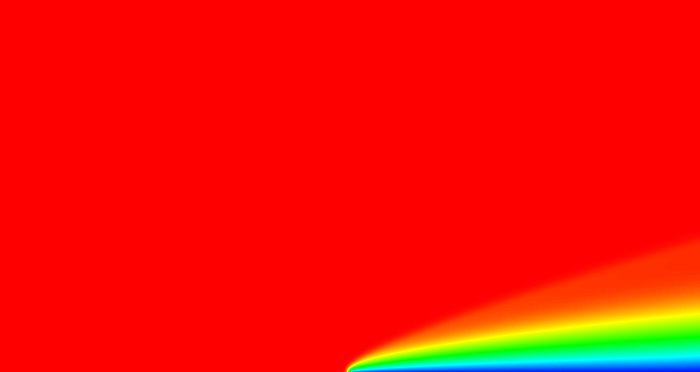
\includegraphics[height = 3cm]{../figures/Jesse/u10.png}}
\caption{Compressible Navier-Stokes for Carter flat plate problem, ${\rm Re}=1000, {\rm Ma}=3.$}
\end{figure}
\end{frame}

\begin{frame}
\frametitle{Camellia: Stiffness Matrix Timing Test}
\begin{itemize}
\item local stiffness matrix computation is \pecosbold{embarrassingly parallel}
\item minimize assembly costs: \pecosbold{spatially local} mesh partitioning
\item timing tests on Lonestar: solve convection-dominated diffusion
\end{itemize}
\vspace{-5mm}
\begin{center}
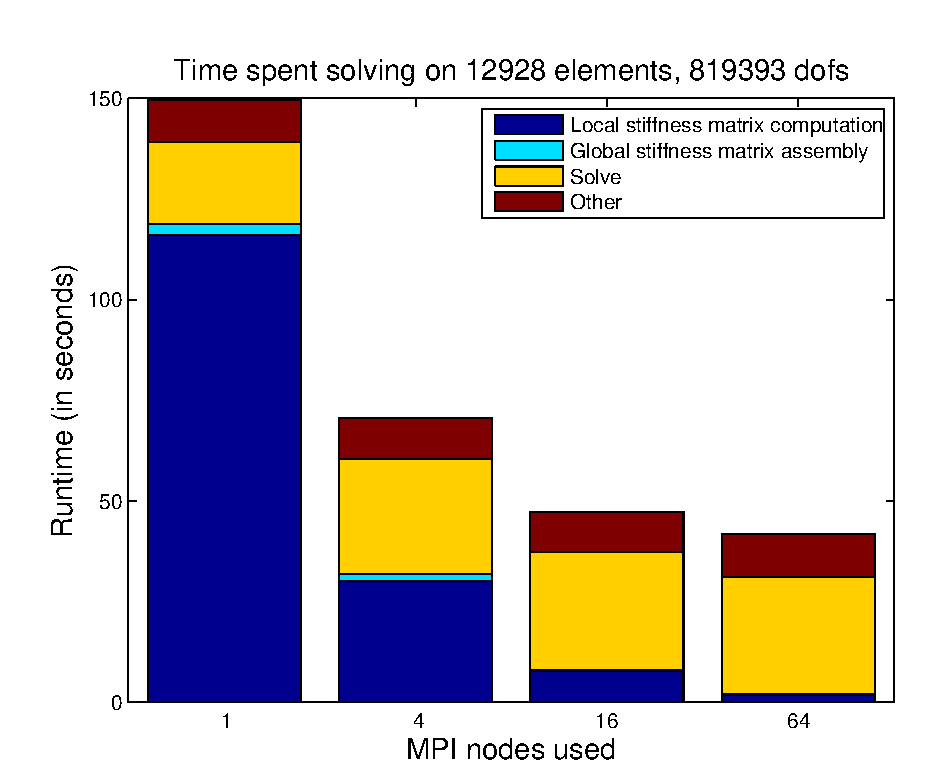
\includegraphics[scale = 0.40]{../figs/scalingFigs/bar_ref3.pdf}\hspace{1cm}
\end{center}
\begin{itemize}
\vspace{-5mm}
\item collaborators working on parallel solvers: Kyungjoo Kim (shared memory architecture),  Maciej Paszynski (distributed memory)
\end{itemize}

\end{frame}


\begin{frame}[fragile]
\frametitle{Camellia: Rapid Specification of Inner Products}
Suppose we have a problem whose graph norm is
\[
\NVRnorm{(v,\vect{q})}_{\rm graph}^{2} = \NVRnorm{v}^{2} + \NVRnorm{\vect{q}}^{2} + \NVRnorm{\NVRpd{v}{x} - \NVRpd{v}{y} + \NVRdiv \vect{q}}^{2}.
\]
\vspace{2mm}
To specify this in Camellia, simply do:
\begin{lstlisting}
VarFactory varFactory;
VarPtr v = varFactory.testVar("v", HGRAD);
VarPtr q = varFactory.testVar("q", HDIV);
IPPtr ip = Teuchos::rcp( new IP);
ip->addTerm(v);
ip->addTerm(q);
ip->addTerm(v->dx() - v->dy() + q->div());
\end{lstlisting}

The bilinear form can be specified similarly.

\end{frame}


%\begin{frame}
%\frametitle{Camellia Details: Stiffness Matrix Computation}
%Recall the problem we solve for the optimal test functions:\\
%For each $e_{i} \in U_h$, find $v_{e_{i}} \in V : (v_{e_{i}},w)_V = b(e_{i},w) \quad \forall w \in V$.\\
%For each $e_{i} \in U_h$, find $v_{e_{i}} \in V : (v_{e_{i}},e_{j})_V = b(e_{i},e_{j}) \quad \forall e_{j} \in V$.\\
%
%\end{frame}

\section{Navier-Stokes} % 7-8 slides
\begin{frame}
\frametitle{Navier-Stokes}
\begin{block}{}
The structure of Navier-Stokes is similar to Stokes:
\begin{itemize}
\item Naive discretizations have similar issues with non-convergence and locking.
\item Can use same elements as for Stokes, but now need to deal with the nonlinearity.
\end{itemize}
\end{block}
\end{frame}

\begin{frame}
\frametitle{Navier-Stokes}
\begin{block}{Existing approaches}
\begin{itemize}
\item Classical pressure-correction methods (Chorin, Temam), velocity-correction methods (Orszag, Karniadakis), and consistent splitting schemes (Guermond and Shen), all of which split the nonlinear time step into a pair of elliptic equations.\footnotemark
\item Guermond and Minev's dimensional splitting, another projection method, which is cheap to compute, only requiring solution of a series of 1D boundary value problems.  (Limited, for now, to axis-aligned parallelepiped meshes.)\footnotemark
\end{itemize}
\end{block}
\addtocounter{footnote}{-1}
\footnotetext{\FootSize \bibentry{Guermond06}}
\addtocounter{footnote}{1}
\footnotetext{\FootSize \bibentry{GuermondMinev2011}}
\end{frame}

\begin{frame}
\frametitle{Navier-Stokes}
\begin{block}{Existing approaches}
\begin{itemize}
\item Cockburn et al. applied LDG to Navier-Stokes, with success for Reynolds numbers up to 100.\footnotemark
\item Evans and Hughes applied divergence-conforming B-splines to Navier-Stokes, with success e.g. for driven cavity problem with ${\rm Re}$ up to 1000.\footnotemark
\end{itemize}
\end{block}
\addtocounter{footnote}{-1}
\footnotetext{\FootSize \bibentry{Cockburn2004}}
\addtocounter{footnote}{1}
\footnotetext{\FootSize \bibentry{EvansHughesSteadyNavierStokes}}
\nocite{EvansHughesUnsteadyNavierStokes}
\nocite{EvansHughesSteadyNavierStokes}
\end{frame}


\begin{frame}
\frametitle{Backward-facing Step}
A classical test case for incompressible flow problems is the \pecosbold{backward-facing step} problem, which has a recirculation region east of the step.  We plan to perform numerical experiments using Stokes, Oseen, and Navier-Stokes.

\vspace{5mm}

\begin{center}
{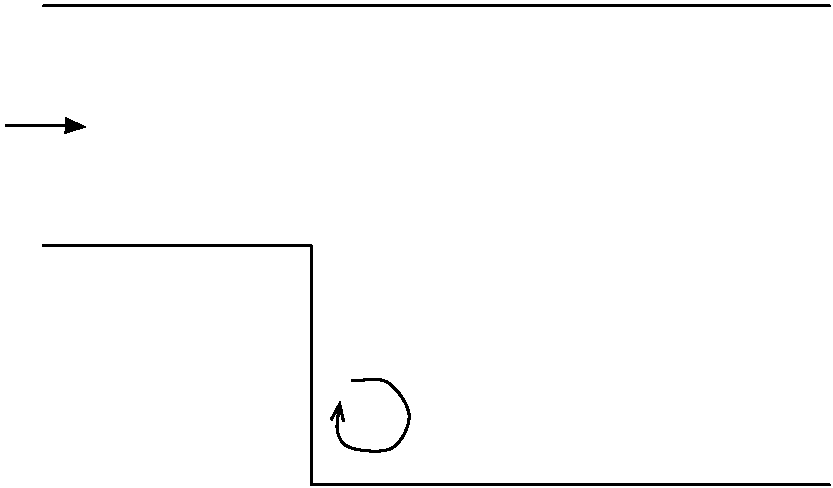
\includegraphics[scale=0.30]{../figures/backFacingStep.pdf}}\hspace{2mm}{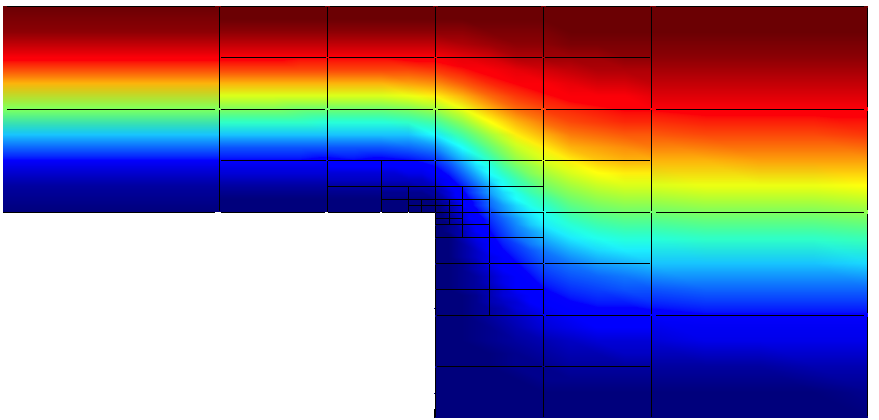
\includegraphics[scale=0.17]{../figures/backFacingStepStreamFunction.png}}
\end{center}

\end{frame}


\begin{frame}
\frametitle{Flow Around a Cylinder}
A classical test case for incompressible Navier-Stokes problems is the flow around a cylinder.\footnote{\FootSize \bibentry{KovasznayCylinder}}  We plan to perform numerical experiments using steady-state Navier-Stokes.

\vspace{10mm}

\begin{center}
{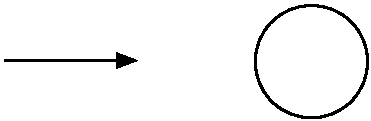
\includegraphics[scale=0.50]{../figures/flowPastCylinder.pdf}}
\end{center}

\pause
At around ${\rm Re}=6$, the flow separates but there is still a steady solution, with symmetric vortices in the wake of the cylinder.  Somewhere above ${\rm Re}=40$, vortex shedding begins (and therefore there is no steady solution).

\end{frame}

% lit. review
% classical problems
\section{Proposed Work} % 3 slides
\begin{frame}
\frametitle{Proposed Work: Area C}
\begin{block}{}
\begin{itemize}
\item Verify convergence rates for the Stokes, Oseen, and Navier-Stokes equations using manufactured solutions.
\item Simulate the classical lid-driven cavity flow and backward-facing step problems using, in turn, the Stokes, Oseen, and Navier-Stokes equations.
\item Simulate flow past a cylinder using the steady-state Navier-Stokes equations.  Time permitting, we will do so with the transient equations as well.
\end{itemize}
\end{block}

\begin{block}{Completed}
\begin{itemize}
\item Verify convergence rates for the Stokes equations using manufactured solutions.
\item Simulate lid-driven cavity flow using the Stokes equations.
\end{itemize}
\end{block}

\end{frame}

\begin{frame}
\frametitle{Proposed Work: Area B}
Design and develop a software toolbox (\emph{Camellia}) for the investigation of DPG problems, with the following features:
\begin{block}{Camellia Features (Completed)}
\begin{itemize}
\item 2D meshes of triangles and quads of variable polynomial order,
\item mechanisms for easy specification of DPG variational forms,
\item $h$- and $p$- refinements, and
\item distributed computation of the stiffness matrix.
\end{itemize}
\end{block}

\pecosbold{Time permitting}, add the following features:
\begin{block}{}
\begin{itemize}
\item curvilinear elements, 
\item meshes of arbitrary spatial dimension,
\item space-time elements, and
\item distributed mesh and solution representation.
\end{itemize}
\end{block}

\end{frame}

\begin{frame}
\frametitle{Proposed Work: Area A}

\begin{block}{}
\begin{itemize}
\item \pecosbold{Completed:} Pose several DPG formulations of the Stokes equations---the velocity-gradient-pressure (VGP), velocity-stress-pressure (VSP), and velocity-vorticity-pressure (VVP) formulations.
\item Pose DPG formulations of the Oseen equations and the 2D incompressible Navier-Stokes equations.
\item \pecosbold{Completed:} Prove the well-posedness of the VGP Stokes formulation for DPG, which has as consequence a guarantee of optimal convergence rates.
\item Time permitting, complete similar proofs for the VSP and VVP formulations.
\item Time permitting, complete similar proofs for the Oseen equations, including a study of \emph{robustness}---analyzing the effects of an increasing Reynolds number.
\end{itemize}
\end{block}

\end{frame}

%===============================================================================
% THANK YOU
%===============================================================================
\begin{frame}
\frametitle{}
\begin{block}{}
\center{Thank you!} \\
\center{Questions?}\\
%For more info:\\
%nroberts@ices.utexas.edu\\
\end{block}
\end{frame}

\bibliographystyle{plain}
{\scriptsize
\bibliography{../DPG}
}

%FOSLS
\addtocounter{framenumber}{-1} % make the next frame # the same as the previous
\begin{frame}
\frametitle{FOSLS\footnote{\FootSize \bibentry{FOSLS1}.}}\nocite{FOSLS2}
First-Order Systems Least Squares (FOSLS), like DPG:
\begin{itemize}
\item first-order system
\item SPD stiffness matrix
\item no need for stabilization terms or flux limiters
\item discrete space only needs to be conforming (no need to satisfy LBB condition, e.g.)
\item minimum-residual method
\item \emph{a posteriori} error \pecosbold{measure} (not estimator)
\end{itemize}
Like DPG, FOSLS provides optimal convergence rates, but it does so in a different norm (typically, the graph norm on the trial space).  Problem-specific approaches to get optimal rates in the $L^{2}$ norm, which DPG manages by virtue of Riesz inversion and a broken test space.
\end{frame}

%Nonlinear derivation, and the Hessian
\addtocounter{framenumber}{-1} % make the next frame # the same as the previous
\begin{frame}
\frametitle{Minimization of the Nonlinear Residual}
As before, we seek to minimize
\begin{align*}
\frac{1}{2} \left(R_{V}^{-1}\left(Bw_{h}-l\right), R_{V}^{-1}\left(Bw_{h}-l\right) \right)_{V},
\end{align*}
but now we allow $B$ to be nonlinear.  The first-order optimality condition then requires that
\begin{align*}
\left(R_{V}^{-1}\left(Bu_{h}-l\right), R_{V}^{-1}B'(u_{h},\delta u_{h}) \right)_{V} = 0, \quad \forall \delta u_{h} \in U_{h}.
\end{align*}
where $B'(u_{h},\delta u_{h})$ is the G\^ateaux derivative of $B$ at $u_{h}$ in direction $\delta u_{h}$.  Then
\begin{align*}
\langle Bu_{h} - l, R_{V}^{-1}B'(u_{h},\delta u_{h}) \rangle = 0 \quad \forall \delta u_{h} \in U_{h}.
\end{align*}
\end{frame}
\addtocounter{framenumber}{-1} % make the next frame # the same as the previous
\begin{frame}
\frametitle{Minimization of the Nonlinear Residual}
\begin{align*}
\langle Bu_{h} - l, R_{V}^{-1}B'(u_{h},\delta u_{h}) \rangle = 0 \quad \forall \delta u_{h} \in U_{h}.
\end{align*}
Now, we can again identify $v_{\delta u_{h}} = R_{V}^{-1}B'(u_{h},\delta u_{h})$ as a test function and note that
\begin{align*}
b(u_{h},v_{\delta u_{h}}) &= l(v_{\delta u_{h}}),
\end{align*}
but notice that now $v_{\delta u_{h}}$ also depends on the solution $u_{h}$.  Linearizing about $u_{h} + \Delta u_{h}$, we have
\begin{align*}
B(u_{h} + \Delta u_{h}) \approx Bu_{h} + B'(u_{h},\Delta u_{h})
\end{align*}
and
\begin{align*}
B'(u_{h} + \Delta u_{h},\delta u_{h}) \approx B'(u_{h},\delta u_{h}) + B''(u_{h},\delta u_{h},\Delta u_{h})
\end{align*}
so that the optimality condition becomes
\begin{align*}
\langle &Bu_{h} + B'(u_{h},\Delta u_{h}) - l,\\
             &R_{V}^{-1}\left( B'(u_{h},\delta u_{h}) + B''(u_{h},\delta u_{h},\Delta u_{h}) \right)) \rangle = 0 \quad \forall \delta u_{h} \in U_{h}.
\end{align*}
\end{frame}
\addtocounter{framenumber}{-1} % make the next frame # the same as the previous
\begin{frame}
\frametitle{Minimization of the Nonlinear Residual}
\begin{align*}
\langle &Bu_{h} + B'(u_{h},\Delta u_{h}) - l,\\
             &R_{V}^{-1}\left( B'(u_{h},\delta u_{h}) + B''(u_{h},\delta u_{h},\Delta u_{h}) \right)) \rangle = 0 \quad \forall \delta u_{h} \in U_{h}.
\end{align*}
Dropping the terms that are second order in $\Delta u_{h}$ and defining $v_{\delta u_{h}} = R_{V}^{-1}B'(u_{h},\delta u_{h})$, we have
\begin{align*}
&\langle Bu_{h} - l, v_{\delta u_{h}} \rangle\\
 &+ \langle Bu_{h} - l, R_{V}^{-1}B''(u_{h},\delta u_{h},\Delta u_{h}) \rangle \\
 &+ \langle B'(u_{h},\Delta u_{h}),  v_{\delta u_{h}} \rangle = 0.
\end{align*}
Rewrite the second term:
\begin{align*}
&\langle Bu_{h} - l, R_{V}^{-1}B''(u_{h},\delta u_{h},\Delta u_{h}) \rangle\\
 &= \left( R_{V}^{-1} (Bu_{h} - l), R_{V}^{-1}B''(u_{h},\delta u_{h},\Delta u_{h}) \right)_{V} \\
&= \langle B''(u_{h},\delta u_{h},\Delta u_{h}), R_{V}^{-1} (Bu_{h} - l) \rangle.
\end{align*}
\end{frame}
\addtocounter{framenumber}{-1} % make the next frame # the same as the previous
\begin{frame}
\frametitle{Minimization of the Nonlinear Residual}
We then have:
\begin{align*}
&\langle Bu_{h} - l, v_{\delta u_{h}} \rangle\\
 &+ \langle B''(u_{h},\delta u_{h},\Delta u_{h}), R_{V}^{-1} (Bu_{h} - l) \rangle \\
 &+ \langle B'(u_{h},\Delta u_{h}),  v_{\delta u_{h}} \rangle = 0.
\end{align*}
Defining $v_{u_{h}} = R_{V}^{-1} (Bu_{h} - l)$, the linearized problem is then
\begin{align*}
b'(u_{h},\Delta u_{h}; v_{\delta u_{h}}) + b''(u_{h},\delta u_{h}, \Delta u_{h}; v_{u_{h}}) = - b(u_{h}, v_{\delta u_{h}}) + l(v_{\delta u_{h}}).
\end{align*}
The solution to this problem minimizes the nonlinear residual $\NVRnorm{Bu_{h}-l}_{V'}$.
\end{frame}

% Assumptions for the well-posedness theorem
\addtocounter{framenumber}{-1} % make the next frame # the same as the previous
\begin{frame}
\frametitle{Technical Assumptions (true for VGP Stokes)}
Under modest technical assumptions (true for Stokes), we have\footnote{\FootSize \bibentry{DPGStokes}}\\
\[
\NVRnorm{Au} \geq \gamma \NVRnorm{u} \implies \sup_{v \in H_{A^{*}}} \frac{b((u,\widehat{u}),v)}{\NVRnorm{v}_{H_{A^{*}}}} \geq \gamma_{\rm DPG} \left(\NVRnorm{u}^{2} + \NVRnorm{\widehat{u}}^{2}_{\widehat{H}_{A}(\Gamma_{h})}\right)^{1/2}
\]
where $\gamma_{\rm DPG} = O(\gamma)$ is a mesh-independent constant, and $\NVRnorm{\cdot}_{\widehat{H}_{A}(\Gamma_{h})}$ is the minimum energy extension norm.\\
\vspace{5mm}
In the next slides, we detail the assumptions.
\end{frame}
\addtocounter{framenumber}{-1} % make the next frame # the same as the previous
\begin{frame}
\frametitle{Technical Assumptions (true for VGP Stokes)}
\[
\NVRnorm{Au} \geq \gamma \NVRnorm{u} \implies \sup_{v \in H_{A^{*}}} \frac{b((u,\widehat{u}),v)}{\NVRnorm{v}_{H_{A^{*}}}} \geq \gamma_{\rm DPG} \left(\NVRnorm{u}^{2} + \NVRnorm{\widehat{u}}^{2}_{\widehat{H}_{A}(\Gamma_{h})}\right)^{1/2}
\]
Define $C$ as the operator arising from integration by parts:
\[
(Au,v)_{\Omega} = (u, A^{*}v)_{\Omega} + \langle Cu, v \rangle.
\]
We split $C$ into $C_{1}$ and $C_{2}$ such that 
\begin{align*}
\langle Cu, v \rangle &= \langle C_{1}u, v \rangle + \langle C_{2}u, v \rangle \\
&= \langle C_{1}u, v \rangle + \langle u, C_{2}'v \rangle
\end{align*}
where $C_{1}u = f_{D}$ corresponds to the Dirichlet BCs imposed. \\
\end{frame}
\addtocounter{framenumber}{-1} % make the next frame # the same as the previous
\begin{frame}
\frametitle{Technical Assumptions (true for VGP Stokes)}
\[
\NVRnorm{Au} \geq \gamma \NVRnorm{u} \implies \sup_{v \in H_{A^{*}}} \frac{b((u,\widehat{u}),v)}{\NVRnorm{v}_{H_{A^{*}}}} \geq \gamma_{\rm DPG} \left(\NVRnorm{u}^{2} + \NVRnorm{\widehat{u}}^{2}_{\widehat{H}_{A}(\Gamma_{h})}\right)^{1/2}
\]
Assumptions:
\begin{itemize}
\item Theorem Hypothesis: with homogeneous boundary condition $C_{1}u=0$ in place, operator $A$ is bounded below in the $L^{2}$-orthogonal component of its null space.
\item $C_{1}$ and $C_{2}$ are defined in such a way that
\[ \left( \langle u,
  C_2^\prime v\rangle = 0 \quad \forall u \: : C_1 u = 0 \right) \implies
  C_2^\prime v = 0.
\]
\item $A$ and $A^{*}$ are surjective.
\item Both graph spaces $H_{A}(\Omega)$ and $H_{A^{*}}(\Omega)$ admit corresponding trace spaces $\widehat{H}_{A}(\partial \Omega)$ and $\widehat{H}_{A^{*}}(\partial \Omega)$.
\item The boundary term $\langle Cu, v \rangle$ arising from integration by parts is definite.
\end{itemize}

\end{frame}
 
\end{document}
